\documentclass[titlesmallcaps, examinerscopy, copyrightpage]{uqthesis}

\bibliographystyle{customIEEEtran}

\usepackage[usenames,dvipsnames]{color}
\usepackage[square,comma,numbers,sort&compress]{natbib}
\usepackage{pdfpages}
\usepackage{graphicx}
\usepackage{eurosym}
\usepackage{appendix}
\usepackage{play}
\usepackage[grey,times]{quotchap}
\usepackage{makeidx}
\makeindex
\usepackage{hyperref}
\usepackage{listings}
\usepackage[nottoc,numbib]{tocbibind}
\usepackage{verbatim}
\usepackage{amsfonts}
\usepackage{array}
\usepackage[acronym,nomain,nonumberlist]{glossaries}
\usepackage{listings}
\usepackage{setspace}
\usepackage[linewidth=1pt]{mdframed}
\usepackage{sverb}
\usepackage{bookmark}
\bookmarksetup{
  numbered, 
  open,
}

\makeglossaries
\renewcommand*{\glossaryentrynumbers}[1]{}

\newcommand{\tick}{\checkmark}
\newcommand{\gtick}{\color{ForestGreen} \tick }
\newcommand{\cross}{$\times$ }
\newcommand{\rcross}{\color{red} \cross }
\newcommand{\runz}{\textsc{Runz}}

\newcommand{\brac}[1]{\left( #1 \right)}
\newcommand*\mean[1]{\bar{#1}}
\newcommand\abs[1]{\left|#1\right|}
\newcommand {\etal} {\emph{~et~al.} }

\DeclareMathOperator*{\median}{median}

\begin{document}
% =====================================================================
% =====================================================================
%%%%%%     TITLE
% =====================================================================
% =====================================================================

\hypersetup{pageanchor=true}
\pdfbookmark{Title}{toc}

\title{Undergraduate Thesis\\ \vspace{0.5 cm} ``Automatic and Assisted Redshift Analysis of Astronomical Objects" }
\author{Samuel Hinton}
\department{EAIT}

\renewcommand{\degreetext}{in partial fulfilment of the Degree Bachelor of Engineering\\ in the
discipline of Software Engineering}

\frontmatter

\titlepage



% =====================================================================
% =====================================================================
%%%%%%     FRONT CONTENT
% =====================================================================
% =====================================================================

\begin{flushright}
Samuel Hinton\\ 41966855\\ 78 Pegg Road, Rocklea, QLD 4106\\
\end{flushright}

\noindent \today \\

\noindent Prof Paul Strooper\\
Head of School\\
School of Information Technology and Electrical Engineering\\
The University of  Queensland\\
St Lucia QLD 4072\\

\noindent Dear Professor Strooper,\\ \\
In accordance with the requirement of the Degree of Bachelor of Engineering (Honours) in the School
of Information Technology and Electrical Engineering, I submit the following thesis entitled:

\begin{center}
  \emph{``Automatic and Assisted Redshift Analysis of Astronomical Objects''}
\end{center}

\noindent The thesis was performed under the supervisor of Dr Vaughan Clarkson and Dr Tamara Davis. I declare that the work
submitted in thesis is my own, except as acknowledge in the text and footnotes, and has not been
previously submitted for a degree at the University of Queensland or any other institution. \\

\noindent Yours sincerely \\ \\ 

\noindent \line(1,0){250} \\

\noindent Samuel Hinton

% =====================================================================

\chapter{Acknowledgements}

I would like to thank my supervisors, Tamara Davis, Vaughan Clarkson and Chris Lidman for their help, assistance and guidance throughout this thesis. I would also like to thank David Parkinson, Conor O'Neill, Michael Childress, David Lagattuta, Syed Uddin, Fang Yuan, Jeremy Mould, Richard Scalzo, Anthea King, Bonnie Zhang and Karl Glazebrook for their feedback, suggestions and testing during this thesis.

% =====================================================================

\chapter{Abstract}

I AM THE ABSTRACT


\cleardoublepage
\hypersetup{pageanchor=true}
\pdfbookmark[chapter]{Table of Contents}{toc}
%\addcontentsline{toc}{chapter}{Table of Contents}

\tableofcontents
\listoffigures
\listoftables

%\printglossary[title=Glossary]
%\addcontentsline{toc}{chapter}{Glossary}

\mainmatter


\chapter{Introduction}

Redshifting measurements form the backbone of many cosmological surveys, and in order to turn spectroscopic measurements into quantified redshifts, a redshifting program is needed. In this thesis, the legacy redshifting software used by the OzDES cosmology team, \runz{}, is replaced with a new, web-based redshifting application developed specifically for their need of an effective algorithm for high redshift and low signal-to-noise data.\\

This report is divided into several sections, with the background and context for redshifting established in Chapter \ref{ch:back} and prior implementations discussed in Chapter \ref{ch:prior}. Those familiar with redshifting and with prior approaches may begin reading from Chapter \ref{ch:req} or Chapter \ref{ch:design}, where program requirements and implementation are respectively discussed.












\chapter{Background}
\label{ch:back}

\section{Usefulness}

With the universe expanding at a current rate of approximately 68 km/s/Mpc \cite{ade2013planck}, electromagnetic radiation travelling through space will increase in wavelength in proportion to the expansion of the space it is travelling through. Quantifying the amount of wavelength shift undergone by light from a distant source, known as redshifting, can be combined with a cosmological model that describes the expansion rate (called Hubble's constant, and denoted $H$), to calculate the distance to the emission object, such that $D = H/v$, where $v$ is the apparent recession velocity of the object given by interpreting the redshift to be akin to common Doppler shift. However, as multiple cosmological models are still being actively considered \cite{davis2007scrutinizing}, it is prudent to keep measurements in the form of redshift measurements, as different cosmological models will translate redshifts to different comoving distances.\\

More formally, the redshift of an observed wavelength is defined with respect to its emission wavelength, such that

\begin{align}
z = \frac{\lambda_{\text{obsv}}}{\lambda_{\text{emit}}} - 1,
\end{align}

and thus an emitted wavelength of 500nm that has been redshifted by $z = 0.5$ would be observed as radiation of wavelength 750nm.

Redshift estimates can be obtained both from spectroscopic and photometric data, each with advantages and disadvantages. Whilst photometric data can be used for fainter objects than currently viable for spectrographs, photometric redshifts do not possess the accuracy of spectroscopic measurements \cite{bolzonella2000photometric}. It is important to note that the OzDES team, for which this thesis was undertaken, are not utilising any photometric redshifts as priors, nor does their instrumentation require photometric data. The OzDES team are using the Anglo-Australian Telescope (AAT) with the AAOmega spectrograph \cite{d2014ozdes}, and thus only require a spectroscopic redshifting solution.

\section{Spectroscopic Features}

Spectrographs provide accurate redshifting due to prominent discernible features in light emissions for galactic objects, where abundant elements such as Hydrogen, Nitrogen and Carbon either emit or absorb at different frequencies. Provided a high enough signal-to-noise ratio in a spectrum, these peaks and troughs can be identified as potential features. Provided a sufficient amount of features, they can be matched to known atomic transitions, whereupon the observed feature wavelength and the known feature wavelength can be compared to determine the redshift of a spectrum. Figure \ref{fig:emission} provides a visual example of a high signal-to-noise spectrum of the Seyfert 2 galaxy NGC 1068 (M77).

\begin{figure}[ht!]
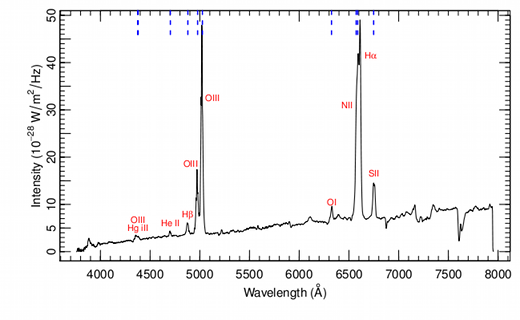
\includegraphics[width=0.75\textwidth]{images/M77_opt_spectrum.png} 
\centering
\caption{A plot of the emission from NGC 1068, with data from the NASA/IPAC Extragalactic Database\cite{nasaDB} and plot courtesy of public R code published by Alastair Sanderson \cite{emission}.}
\label{fig:emission}
\end{figure}

\section{Spectrum types}

\textcolor{red}{ADD SOME SPECTRA, QUASARS< EMISSION TYPES, ETC.}


\section{Common Complications}

High quality spectrum, with well defined and multiple emission features, such as shown in Figure \ref{fig:emission}, become progressively less common with increasing redshift, due to increasing distance to emission object and thus lower light intensity. As such, redshifting algorithms have to employ data reduction and matching techniques specifically designed to marginalise potential error and account of known complications. In this section, several complications to the redshifting process that have been actively encountered in this thesis will be discussed. Ideas on how to marginalise or reduce these complications will be discussed in the implementation section of this thesis. The OzDES data workflow currently includes a separate data reduction pipeline which aims to account for many of these factors in the data before being sent for redshifting to reduce data traffic and thus lower network overhead, however a lack of finalisation in the data reduction pipeline's capabilities means that all major concerns will be detailed in this section.

\subsection{Planetary Atmospheric Interference}

Given that the Anglo-Australian Telescope is located on the ground in Australia, interference from the night sky has to be dealt with. The sky itself, possessing both necessary ingredients of light and atoms, has its own emission spectrum which all spectrographs will detect \cite{Meinel1950Emission}. By observing the night sky without a background emission source, the night sky can be subtracted out of target spectrum, however this process can be imperfect in implementation due to spectrograph error, optical distortion and variability of the sky's emission and absorption spectrum \cite{Kelson2003Optimal}. Figure \ref{fig:night} shows the sky spectrum above Mauna Kea to illustrate the intensity of many features found in the night sky.

\begin{figure}[ht!]
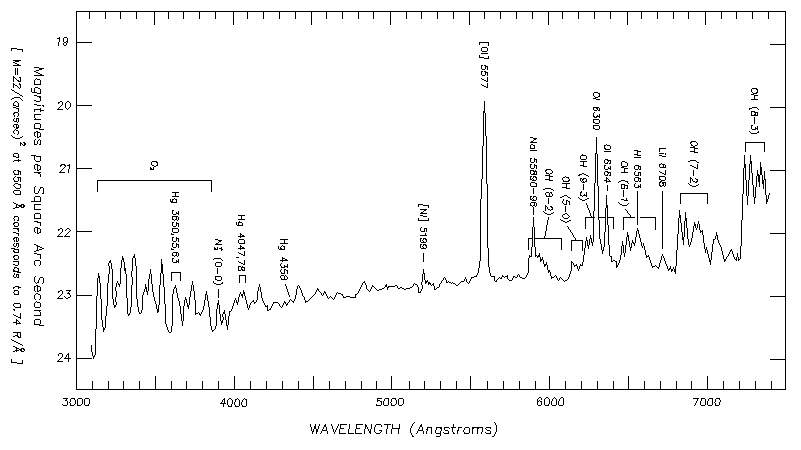
\includegraphics[width=0.9\textwidth]{images/om-nskyvis.jpg} 
\centering
\caption{A plot of the night sky emission above Mauna Kea from the Canada-France-Hawaii Telescope Observatory Manual \cite{night}. Please see the manual for data sources and further attribution.}
\label{fig:night}
\end{figure}

\subsection{Planetary Atmospheric Correction}

A simple consideration when examining spectrum is that the wavelengths being recorded are the wavelengths of light in air (for a ground based telescope). Due to the non-linear nature of converting air wavelengths to vacuum wavelengths, this is often done via interpolating conversions from empirical tabular data sets determined from controlled laboratory experiments \cite{morton1991atomic}.

\subsection{Heliocentric velocity}

With the accuracy of spectroscopic redshifting, the planet's heliocentric velocity (velocity relative to the sun) provides a significant enough contribution that it needs to be corrected for \cite{colless20012df,baldry2014galaxy}. This can be done by calculating the relative velocity of the Earth in its solar orbit relative to the object being observed, and subtracting the appropriate redshift contribution. Given that multiple observations from different times in the year can be stacked and presented a single spectrum to be redshifted, heliocentric velocity corrections should be applied in the data reduction pipeline instead of in the redshifting algorithm.

\subsection{Cosmic Rays}

Cosmic rays are the name given to extremely high energy particles travelling in space. Cosmic rays are generally massive particles such as protons moving at relativistic speeds, often due to acceleration in a supernova \cite{ackermann2013detection}. Due to their colossal energy, in which the record is approximately $3\times10^{8}$ TeV (23 million times as energetic as the maximum energy rating of the Large Hadron Collider when set to reopen in 2015 \cite{lhc}), a single strike by a cosmic ray will appear as an extraordinarily thin and powerful emission line in a spectrum. Cosmic ray impacts look similar to strong emission lines, and thus a large problem I had to solve in the processing was to be able to remove cosmic rays without removing important emission features. The effect of a cosmic ray in a spectrum can be seen in Figure \ref{fig:cosmic}, where the massive peak near 5700{\AA} is a cosmic ray and not a true feature.


\subsection{Equipment Miscalibration}

Most modern spectrographs, including the AAOmega spectrograph, feature more than one digital camera (charge-coupled device, CCD) with which to measure a spectrum. Different CCD's are more sensitive to different wavelength ranges of light, and so in order to expand the wavelength range of the devices, CCD's with different range sensitivities are used.  Specifically, the AAOmega spectrograph features both a red and a blue arm in the spectrograph, and light is divided to en-route to the detector \cite{aaomega}. Problems can arise when trying to merge the separate sensor results into a final spectrum, with the possibility of spectral arms (with different CCD's) being miscalibrated. Miscalibrating the relative strength of the CCD's can lead to dichroic jumps in the spectrum, which can be easily mistaken for emission features. A sample spectrum has been provided for illustrative purposes, and the dichroic jump can be clearly seen at approximately 5800{\AA} in Figure \ref{fig:jump}


\subsection{Physical Interference}

Difficulties in redshifting spectrum can also arise when physical interference in the spectrum can remove or hide useful features. A prominent cause of this interference is intergalactic and intragalactic dust and particulate, which will interact with light and often result in absorption troughs in the measured spectrum. Not only do these introduced features not belong to the object we are trying to be observe, these absorption features can remove useful matching features of the base object if the absorption occurs at the same wavelength region as the expected feature. An example of unusual absorption features added to a spectrum from dust interaction can be seen in Figure \ref{fig:dust}, particularly in the first and third broad peaks, centred around 4400{\AA} and 5500{\AA} respectively.




\begin{figure}[ht!]
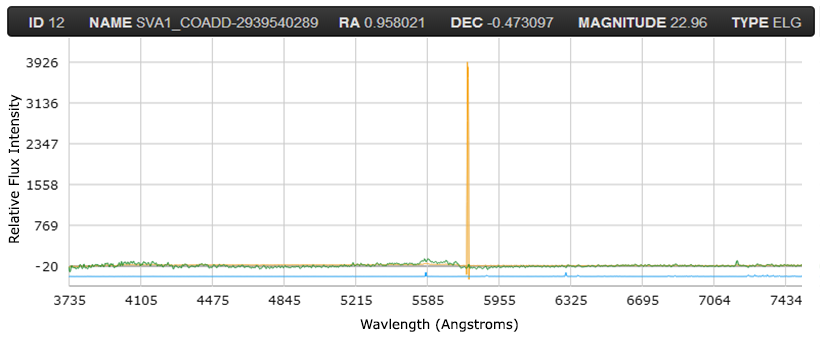
\includegraphics[width=1\textwidth]{images/CosmicRay.PNG} 
\centering
\caption{AAOmega spectrum of an emission line galaxy and a cosmic ray hit. Spectrum provided courtesy of Conor O'Neill and graphed using the developed thesis software prototype, with cosmic ray jump clearly visible at approximately 5700{\AA}.}
\label{fig:cosmic}
\end{figure}

\begin{figure}[ht!]
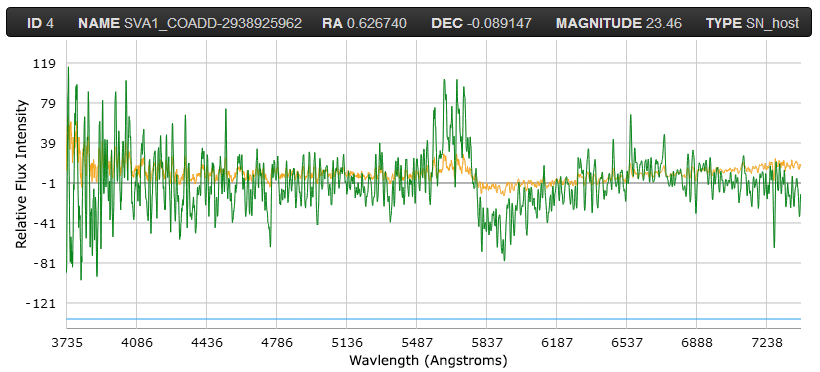
\includegraphics[width=1\textwidth]{images/jump.PNG} 
\centering
\caption{AAOmega spectrum of a supernovae host galaxy, spectrum provided courtesy of Conor O'Neill and graphed using my thesis software prototype, with the dichroic jump clearly visible at approximately 5800{\AA}.}
\label{fig:jump}
\end{figure}

\begin{figure}[ht!]
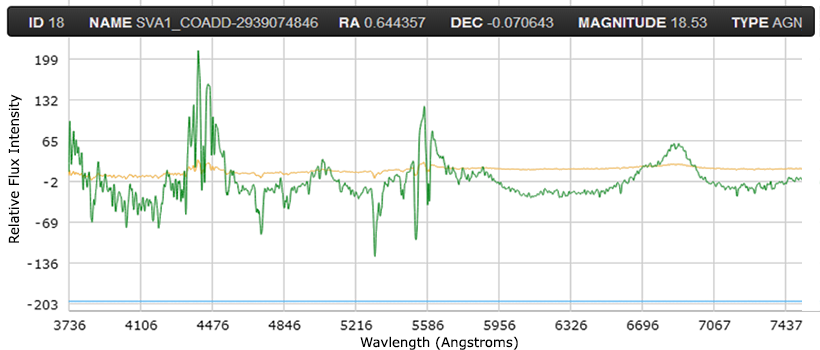
\includegraphics[width=1\textwidth]{images/dust.PNG} 
\centering
\caption{AAOmega spectrum of a quasar, spectrum provided courtesy of Conor O'Neill and graphed using the developed thesis software prototype, with absorption troughs not found in quasar template spectra scattered throughout the spectrum below from 4100{\AA} to 5900{\AA}.}
\label{fig:dust}
\end{figure}































\chapter{Prior Methods}
\label{ch:prior}

There are many prior approaches available for review, catering to a wide range of astronomical objects and varying observational distances and magnitudes. In this section, I will review several of the software packages used by large cosmology surveys.

\section{Implementations}

\subsection{RVSAO 2.0}

The RVSAO 2.0 software package is a highly used redshifting and templating software package, containing programs to perform cross correlation redshifting (\verb+xcsao+), feature matching (\verb+emsao+), template building (\verb+sumspec+) and more. The main program used for redshifting, \verb+xcsao+, is of main interest to this literature review, as the matching algorithm for the \verb+emsao+ program does not perform better in either high or low signal-to-noise spectrum than \verb+xcsao+ \cite{kurtz1998rvsao}.

Power spectrum techniques such as cross correlation were first used to analyse spectrum by Tonry and Davis in 1979 \cite{tonry1979survey}, digitalising the analog techniques used by Griffin in 1967 \cite{griffin1967photoelectric}. The \verb+xcsao+ software program follows the methods outlined by Tonry and Davis, and has been in use since 1985 \cite{kurtz1998rvsao}. The specific algorithms of the \verb+xcsao+ program are outlined by Kurtz and Mink \cite{kurtz1998rvsao}, and are summarised below.

The software takes a spectrum with a user defined wavelength range, subtracts continuum, and - depending on the configuration of the program - can also remove emission or absorption lines. The spectrum is then apodized to remove ringing after a Fourier transform is preformed, zero-padded to remove potential artifacts after Fourier transformation, and Fourier filtered to try and improve the signal-to-noise ratio via a bandpass filter. The spectrum and each potential matching template is then rebinned, and cross correlated around a user defined redshift estimate to find the redshift of maximum correlation. The goodness of the fit is determined by the size of main peak fit, and the final redshift and confidence of fit are supplied to the user as the program's final result.

Whilst the cross correlation algorithms in use are tried and tested, the ease of use of the RVSAO 2.0 software package leaves much to be desired. Operating only in command line and without any interactive user input, the 2010 release of the \verb+xcsao+ program takes up to 67 input parameters \cite{parameters}, making intuitive use of the program impossible and introducing experience based technical overhead to cosmology groups attempting to use the software.

\subsection{2dF Galaxy Redshift Survey}
The 2dF Galaxy Redshift survey was designed to measure the redshift for approximately $250\;000$ galaxies using the Anglo-Australian Telescope \cite{colless20012df}. The algorithms used in the analysis of the spectroscopic data include data reduction and redshift estimation, where on the latter will be investigated in this review, as the data reduction pipeline used by OzDES is outside the scope of this thesis.

The matching algorithms used by the 2dF team are also descendent from the algorithms put forth by Tonry and Davis \cite{tonry1979survey}, where (like RVSAO 2.0), redshift determination can be achieved both by cross correlation methods and feature matching \cite{colless20012df}. The program performs several steps of preprocessing on the spectrum, where detected atmospheric lines are removed via interpolation over a spectrum window, continuum is removed via the subtraction of a fitted sixth degree polynomial, and points more than five times the root-mean-square (rms) deviation from the mean are removed from the spectrum. The spectrum is rebinned, apodized and then Fourier transformed. The transformed spectrum is then filtered with an exponential filter to remove noise and subtract continuum further. The result of this filter is then cross correlated with all available templates, with the greatest cross correlation peak determining the final redshift.

Emission line matching is done via fitting tight Gaussian peaks around strong emission features. The three strongest emission lines in the spectrum are tested against common strong emission lines, such as triply ionized oxygen (O$_{\rm{III}}$), the hydrogen beta transition (H$_\beta$), the hydrogen alpha line (H$_\alpha$), or the doubly ionized nitrogen line (N$_{\rm{II}}$). If the emission lines are found to match these common transitions, the redshift can be determined via comparison of the detected peak wavelengths and the rest frame wavelengths.

After determining the final redshift, the spectrum is then displayed to the user, who then has the choice of accepting the suggested redshift or manually fitting the spectrum themselves. The visual feedback provided by the 2dF software marks a large improvement in usability over the RVSAO 2.0 software package.



\subsection{SDSS DR8 $\chi^2$ fitting}

The Sloan Digital Sky Survey (SDSS) has been active since 2000, and latest data release - data release 10, includes spectroscopic measurements for over one million objects \cite{SDSSIII}. This review will concentrate on the eighth data release (DR8) \cite{aihara2011eighth}, in which the redshifting algorithms utilised are discussed more in depth. Prior to DR8, the redshifting algorithms used by the SDSS team included standard cross correlation techniques similar to those of 2dF and RVSAO 2.0, with $\chi^2$ algorithms also available \cite{sdss6}. In DR8, the cross correlation method was removed in favour of the $\chi^2$ fitting, as they gave the same results for approximately 98\% of spectrum \cite{aihara2011eighth}. Whilst the reasons behind the decision to move to $\chi^2$ analysis instead of cross correlation is not elucidated in the data release, the $\chi^2$ approach does have an advantage in requiring less processing of spectra.

The $\chi^2$ matching process is simpler than the cross correlation algorithm, and input spectra have a sky mask applied to zero weight skylines, and then, for a range of viable redshifts, the $\chi$ difference for each template in the catalogue is determined, where the $\chi^2$ difference is defined as:

\begin{equation}
\chi^2_z = \sum_i \left(\frac{t_{iz} - \mu_i}{\sigma_i} \right)^2,
\end{equation}

where the index $i$ denotes the $i$th data point, $t_iz$ is the value of the template's $i$th point at a shifted redshift of $z$, $\mu_i$ is the $i$th value of the spectrum intensity, and $\sigma_i$ is the $i$th value of the error spectrum. As of the eighth data release, the redshift increment in each step is 138 km s$^{-1}$, and all galactic templates are checked between a redshift value of $-0.01 \geq z \leq 1.00$. Whilst this method is certainly mathematically simpler than many alternate algorithms, I am concerned over the lack of detail given in the examined papers algorithm review about catering for factors such as varying normalisation over redshift ranges, as proper $\chi^2$ analysis requires normalisation such that the $\chi^2$ difference is minimised and any algorithms or methods used to do such minimisation are not detailed.



\subsection{\textsc{AUTOZ}}

The \textsc{AUTOZ} program written by Ivan Baldry is an IDL based algorithm to provide redshift estimation for the Galaxy and Mass Assembly (GAMA) team \cite{baldry2014galaxy}. My analysis of the matching algorithm finds many similar steps to previously reviewed programs. \textsc{AUTOZ} applied flux corrections to account for non-uniform spectroscopic sensitivity, removes bad data points, subtracts continuum via rejected polynomial fitting and subtraction of a smoothed median filter, apodizes the spectrum with a cosine taper, divides the spectrum intensity by the spectrum variance squared and finally oversamples and rebins the spectrum. This final spectrum is then Fourier Transformed and cross correlated with a range of provided templates, where the highest cross correlation peaks are used to determine the best fitting redshift and template.

Unlike the 2dF program, which allows users to manually verify the automatically determined redshift and then pick their own redshift if unsatisfied, the \textsc{AUTOZ} program provides no interactivity or manual verification of redshifts. Whilst the program does allow a substantial number of input parameters to be specified that effect the matching algorithm, that is the extent of user input. Furthermore, the \textsc{AUTOZ} application is developed for a specific and restricted set of astronomical objects due to the target survey population of the GAMA survey.

\section{Trends and Caveats}

Given that the algorithms reviewed have been arranged in chronological order, it can be seen first off that emission line matching via feature identification has not been used in the more modern implementations. As discussed in the review of RVSAO 2.0, emission line matching has been found to be inferior to cross correlation matching for both high and low signal-to-noise data. Given the suitability of emission line matching mainly to high quality emission type galaxy spectrum, this technique would be the least applicable to the large amount of low signal-to-noise data being gathered by the OzDES team.

When looking at cross correlation techniques, it can be seen that similarities in the matching algorithms of all four reviewed programs indicates that the core methodology has not changed significantly since it was first implemented by Tonry and Davis \cite{tonry1979survey}. The $\chi^2$ method of matching redshifts is only mentioned by the SDSS team, however they found it simple and useful enough to completely remove their cross correlation algorithms in favour of the $\chi^2$ approach. The success of that approach warrants an investigation and implementation of a $\chi^2$ matching algorithm in the thesis project, along with an implementation of a cross correlation based matching algorithm.


\section{Current OzDES Approach}

Currently the OzDES team is using legacy software called \runz{} to perform redshift estimates. This software provides two separate matching algorithms, respectively using cross correlation and feature matching similar to the RVSAO 2.0 software package. Similar to the 2dF software, the user can select a manual redshift if unsatisfied with the best automatically determined redshifts. Users can find manual redshifts by virtue of marking spectral features as specific transitions via a simplistic visual interface illustrated in Figure \ref{fig:runz}, and can then perform a tightly constrained  automatic fit to shift the selection to the maximum cross correlation. The OzDES team is seeking replacement software due not only to the low accuracy of the automatic redshifting algorithm in \runz{}, but also due to the legacy nature of the software, which requires various archaic dependencies, C-shell, in addition to a steep learning curve. Modifying \runz{} to address these issues is not desired due to the unfortunate state of the code base after over a decade of revisions and additions. The next chapter will state the requirements of any replacement software in order to address the current disadvantages and issues relating to the installation and use of the current \runz{} software program.

\begin{figure}[ht!]
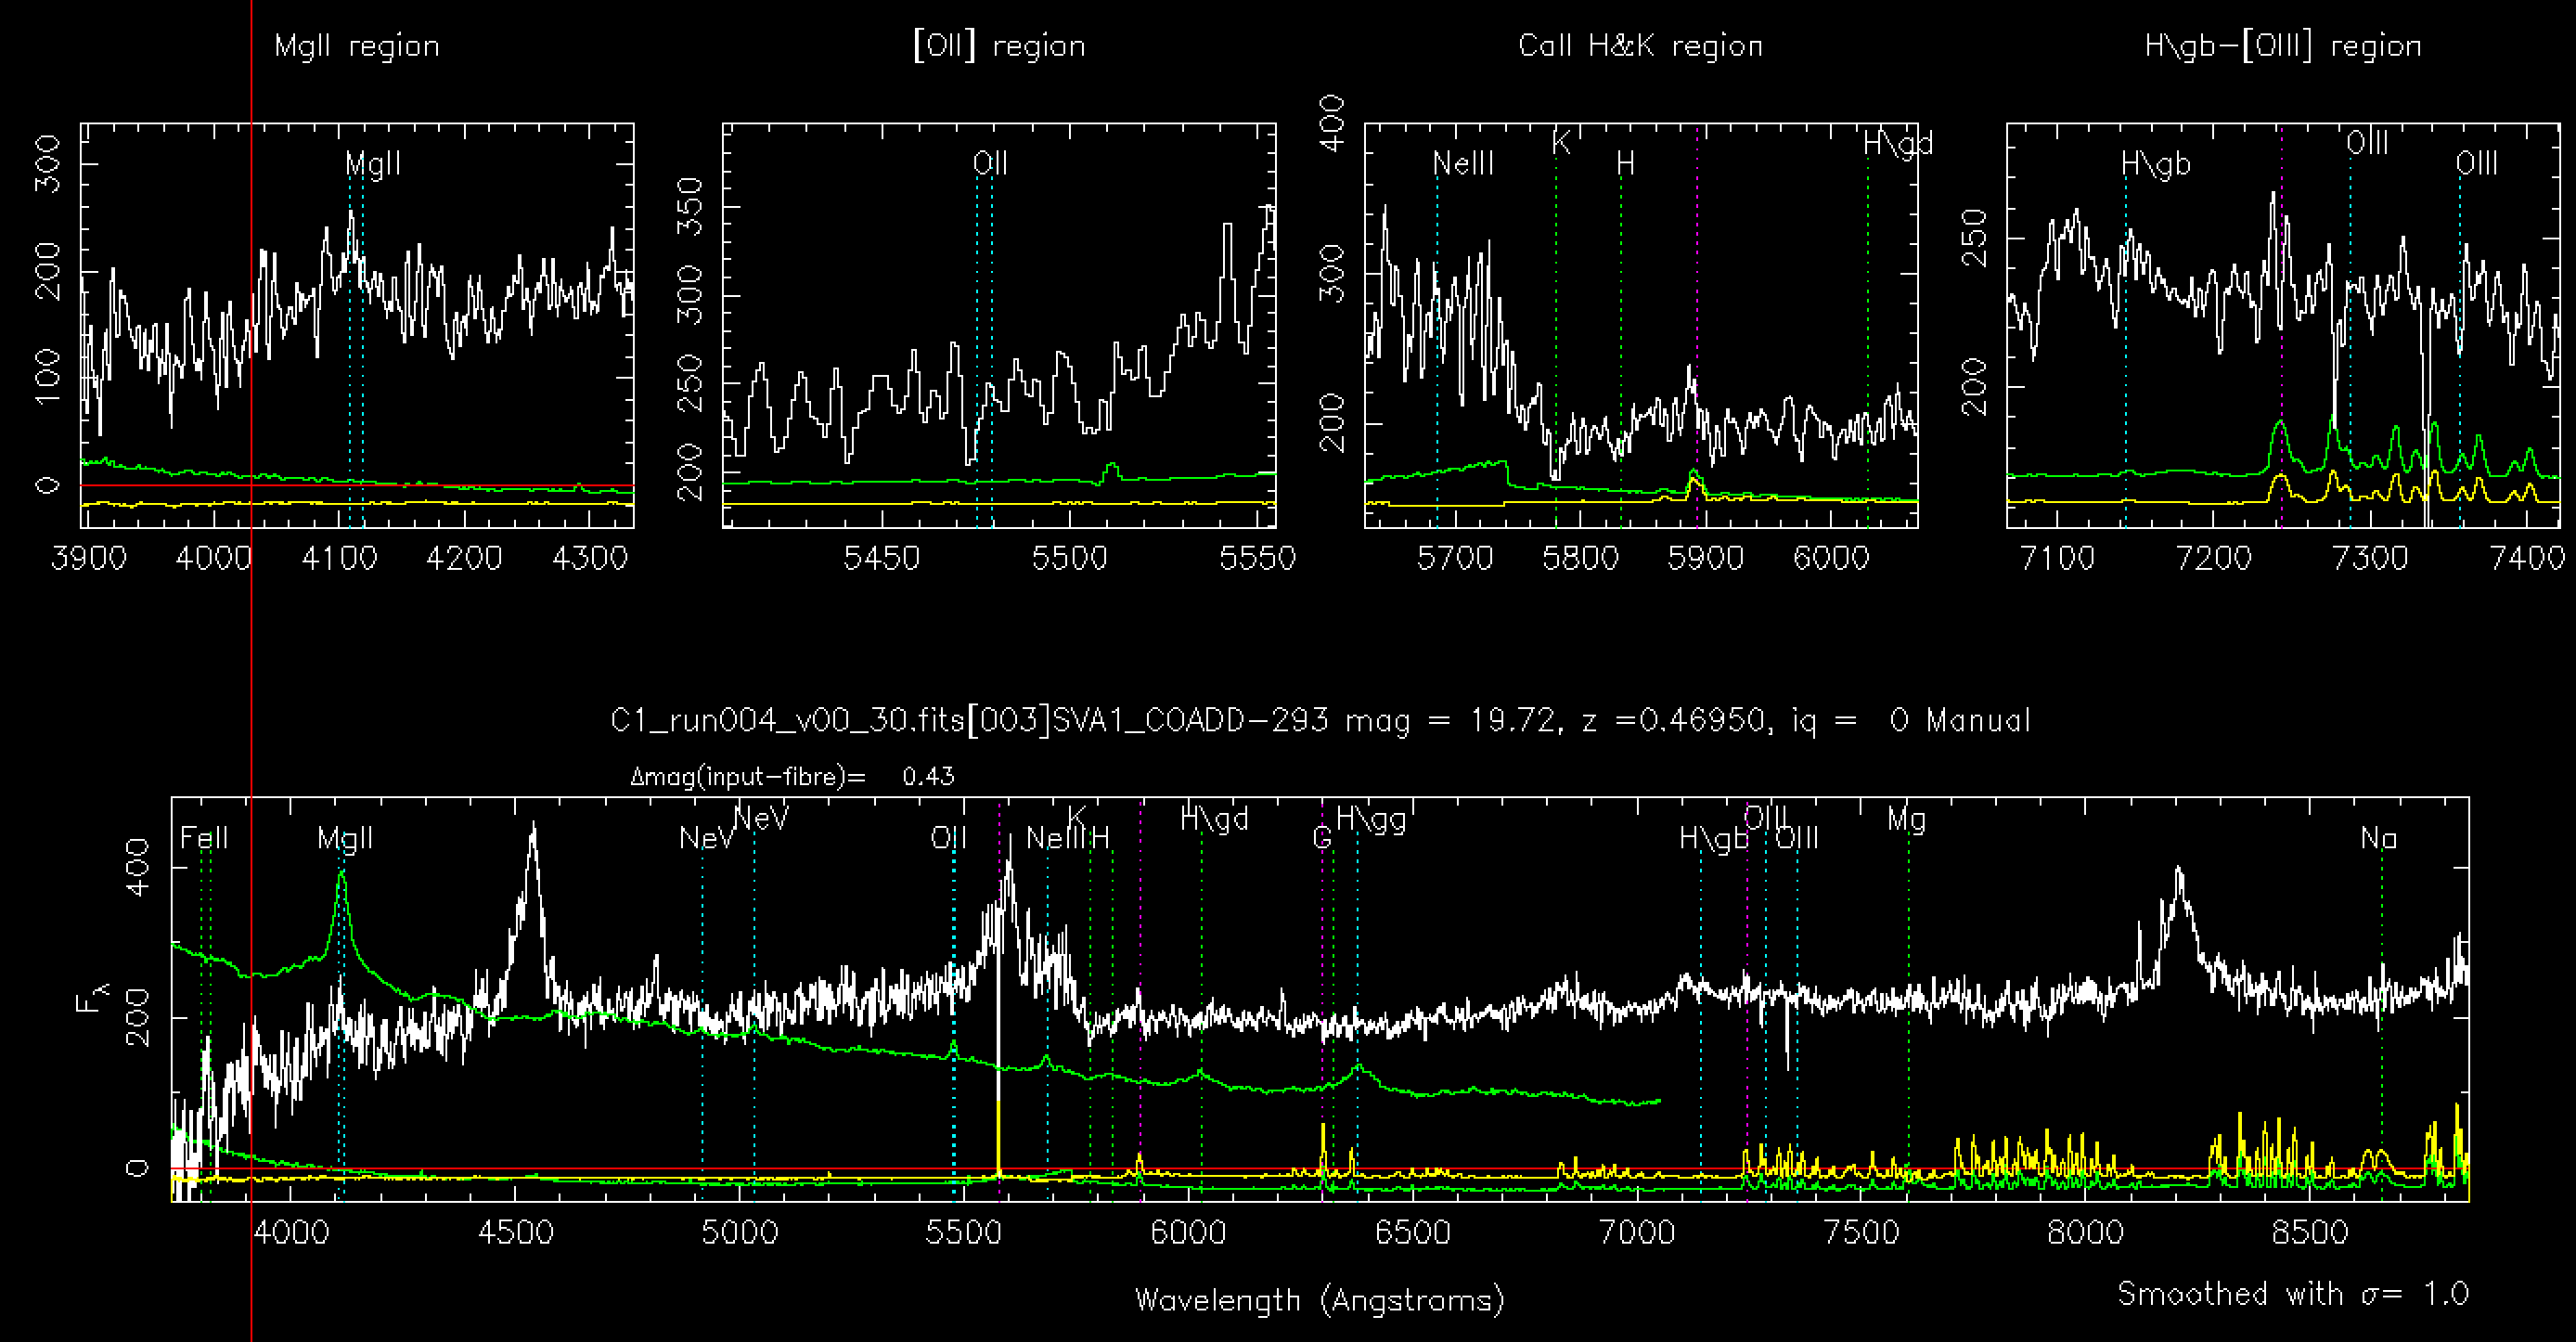
\includegraphics[width=1\textwidth]{images/RunzScreen.PNG} 
\centering
\caption{A screenshot of the \runz{} application in use. The four top plots represent detailed callout sections, with the full spectrum shown in white in the bottom plot. The perspective template to match to is shown in green in all plots. The red line through the image serves as the cursor for \runz{}, where spectral lines are marked at the current cursor via keyboard shortcuts, which are displayed in a background terminal window to which \runz{} displays output.}
\label{fig:runz}
\end{figure}



% =====================================================================

\chapter{Requirements}
\label{ch:req}

Consultation with the OzDES team produced a list of usability and functional requirements that need to be met before the thesis program can be considered a viable replacement for \textsc{Runz}. In this section, these requirements are discussed under the general categories of algorithm matching performance, computational performance, usability, and integration features.
\section{Algorithm Performance}

Every night of observation at the AAT can produce four thousand spectrum. Each of these spectrum needs to be analysed by a member of the OzDES team to ascertain two values: a redshift estimate and a quality of estimate, as represented an integer range from 1 (illegible spectrum) up to a quality of 4 (99\% confidence in results). The desired goal for the algorithm matching performance is to be able to agree with manual matching for 90\% of spectrum, where the user has selected a quality of matching to be 4, indicating a high quality spectrum and defined spectral features. Whilst other surveys and their matching algorithms have managed to attain over 90\% accuracy prior to this thesis, the algorithms developed for OzDES will need to be able to perform under circumstances of much lower signal-to-noise than previous surveys and need to be effective at matching a wider range of astronomical objects.

The absolute lower bound for accuracy during redshift estimate is to match the performance of the \textsc{Runz} application. Thus, analysis of algorithm performance will necessarily involve comparison to the performance of automatic matching via \textsc{Runz}.

Performance is looked to be gained over that of \runz{} in matching all targets, where quasar matching is a known weakness in prior algorithms and \runz{} due to the high redshift estimations and broad features of quasar spectrum. Generalising this requirement, any developed matching algorithm has to give high performance over a wide variety of traditional and exotic astronomical objects.

\section{Computational Performance}

The software developed needs to be accessible to end users without the aid of dedicated cluster or supercomputer stations. Memory and CPU utilisation of the application should fit within acceptable bounds such that the application can be executed without issue on computer hardware featuring dual core processors and 2GB of RAM. This is a soft goal, in that it is desired but not necessary for software adoption, however great care needs to be taken to ensure that the vast majority of expected users possess the hardware required to run the program without issue.

\section{Usability}

\subsection{Installation}

Given the legacy state of the current OzDES redshift matching software, \textsc{Runz}, initial installation of the software program and its required dependencies is an onerous task, and has taken in some cases over a week of effort before the program was in a usable state. A requirement for adoption by the OzDES would be significant improvements in the installation process. Ideally, installation should be achieved by a self-contained  single-file installation package, with any required dependencies installed either automatically or with minimal fuss.

Whilst cross-platform support is not a requirement for the OzDES team, it would be a desirable feature, as previous applications required a a Mac or Linux distribution.

\subsection{Updating}

In line with the request for minimal maintenance and human intervention, a further goal of this thesis will be to produce software that updates either automatically, or via a simple prompt to the end user. It is expected that at no point in any update process would a user have to manually updated any dependencies, or manually configure or replace program content, such as binary files.

\subsection{Uptake}

A final large issue that effects new users to \textsc{Runz} is the steep learning curve of the program. As briefly mentioned previously, \runz{} features a simple visual interface. This interface consists of cursor tracking, plot rendering and keyboard shortcuts, with none of the modern hallmarks and interactivity the define modern user interfaces. Furthermore, keyboard shortcuts, program output and help text is all displayed in a separate terminal window, creating an unpleasant disjoint between information location and the respective visual detailing of that information on the plots. The lack of modern control schemes and unintuitive segregation of information and visual content makes \runz{} unintuitive for new users, and the OzDES team are looking for an interactive and intuitive user interface in replacement software.

In addition to the usability of the interface in general, \runz{} provides limited screen options, restricting users to viewing a spectrum in full (as shown in Figure \ref{fig:runz}), or to seeing a plot detailing redshifts for all spectrum in the input file. It provides no way to inspect template files by themselves, no options or settings screen, and no overview screen by which to view multiple spectrum, either in tabular or graphical format.

\subsection{Automation}

Although not a strict requirement, members of the OzDES team have enquired about the potential to automate the program, so that it can be inserted in the data pipeline without hassle. Given that manual data checks will still need to be performed, this requirement is an attempt to reduce time spent gathering relevant data files and waiting for the algorithm to redshift spectrum before manually verifying the automatic results. As such, an objective for the algorithm is to match at a speed greater than that of a user manually matching spectrum, to ensure that users do not find themselves waiting upon automatic matching to determine a redshift estimate.

\subsection{Retention}

The final usability requirement given by the OzDES team was to ensure that work could not be lost accidentally during the redshifting process. \runz{} achieves this goal via saving results straight to hard disk during redshifting, and similar levels of data retention need to apply for any developed application such that unexpected failure of the application, either through internal exceptions or being accidentally closed by the user, does not result in lost data and having to re-redshift spectrum.




\section{Integration}

The final requirement for the program is in being able to integrate with the existing systems in place used by the OzDES team. Specifically, the program would need to take inputs of singular observation runs after data reduction, and be able to take data files created by aggregation of multiple observations by the OzDES team. The results produced by the program then need to be a consistent, machine readable format, suitable for easy digestion into a database system.










































\chapter{Design and Tool Decisions}
\label{ch:design}

The requirements discussed in the previous chapter allow comparison of multiple possible development pathways. In this section, high level design decisions are laid out in terms of their advantages and disadvantages. 

\section{Languages}

\subsection{Python}

Python is a versatile, open-source, high-level programming language that supports the programming paradigms of object-orientated, structured, dynamic, functional and procedural coding \cite{Python}. It is gaining popularity quickly in the astronomical community, with 50\% of respondents to an astrostatistics survey specifying Python as their programming language of choice as of 2014 \cite{PythonPop}.

\subsubsection{Advantages}

\begin{itemize}
\item \textbf{External Libraries:} The greatest advantage of Python is the abundance of  high quality external python libraries available for academic use. In particular, the Astropy library provides programmers with a massive amount of relevant scientific methods, data analysis tools and data visualisation tools that can enormously simplify workflow processes \cite{astropy}. Other libraries, such as NumPy, focus on bringing speed to Python via wrapping compiled FORTRAN or C++ code in a Python wrapper, aiming to leverage the easy programming of Python with the efficiency of low-level languages \cite{numpy}.

\item \textbf{Platform agnosticism:} Python is available cross platform, and thus a Python implementation would be platform agnostic provided that any external libraries that use precompiled binary wrappers have versions available both unix based operating systems and Windows.

\item \textbf{Readability:} A final advantage of using the Python language is it's readability. Given that it is expected that multiple people will maintain the project and potentially contribute to it in the future, it would be highly beneficial if code written is easy to understand by readers without an in-depth technical background.
\end{itemize}
  

\subsubsection{Disadvantages}

\begin{itemize}
\item \textbf{Dependency Management:} Unfortunately, the large number of available Python libraries can often lead to dependency conflicts, where specific libraries require different versions of Python to work. In addition to this, a Python version chosen for the project would need to be installed onto all user's computers (as Python is interpreted), and some users may be reticent to installing a different version of Python for a single application.

\item \textbf{Advanced User Interface:} Whilst there are dozens of graphical user interface (GUI) libraries written for Python \cite{PythonGUI}, it is often the case that these libraries are platform dependent or require large amounts of code to create interactive interfaces. Given my inexperience with the most modern Python GUI, additional time would have to be devoted to selecting the best library available and learning how to us it.

\item \textbf{Updating:} Automatic updating would be difficult with a Python application in the circumstance of attempting to upgrade dependencies. As users may be utilising application dependencies for other projects, it is impermissible to update dependencies without notifying the user. In the case where other programs require a different version of an external library, unless the user decides to create a new Python installation, they cannot update the project.

\end{itemize}

\subsubsection{Verdict}

Despite the issues relating to external dependencies and unfamiliarity with developing Python user interfaces, the fantastic libraries available make Python a promising pathway to consider.


\subsection{C++}

C++ is a low-level, compiled programming language that is known for library support and high-speed execution \cite{cpp}.

\subsubsection{Advantages}
\begin{itemize}

\item \textbf{Speed:} Given that C++ is a low-level, compiled language, its execution speed is significantly faster than interpreted languages like Python. Given the numerical complexity and large data sizes found in many astronomical tasks, the speed of C++ can be required for high performance domains. Whilst this is obviously a boon in any circumstance, it should be noted that this project does not strictly posses an efficient high-performance computing requirement, and that many libraries in Python (such as NumPy) to some extent negate the speed benefit of C++.

\item \textbf{Maturity:} C++ is a mature ISO-standard language, and thus code written for C++ is highly likely to remain standards compliant over future revisions. As a counter example to this, consider the fragmentation in the Python code base which is split between versions 2.7.8 and 3.4.1 due to large code changes \cite{pythonDownload}.
\end{itemize}

\subsubsection{Disadvantages}
\begin{itemize}

\item \textbf{Fewer Modern Libraries:} Given the low popularity of C++ in astronomy, regularly updated and comprehensive libraries are few and far to be found. Whilst general scientific and signal processing libraries exist, the list of high quality C++ libraries pertaining to astronomy libraries is not as comprehensive as available in Python. In addition, many C++ libraries are platform dependent, locking down platform choices.

\end{itemize}

\subsubsection{Verdict}
In light of the fact that the speed advantages of C++ over interpreted languages like Python are largely removed due to Python wrappers over compiled binaries, the only compelling reason to implement the program in C++ is unconvincing.


\subsection{IDL}

IDL is a programming language developed by Exelis specifically for scientific computing, aiming to be easy to use, easy to read, and concise \cite{idl}. 

\subsubsection{Advantages}
\begin{itemize}
\item \textbf{Built in functions:} Being a scientific computing language, IDL comes with a large amount of built in functions that lowers the requirement for external dependencies for complex mathematical functions, visualisation and data manipulation. Given the scientific context of IDL, it also has built in support for array operations not found in many other languages.
\item \textbf{External libraries:} IDL is still a common choice for astronomical projects \cite{PythonPop}, and this is in large part due to comprehensive astronomical library repository available from NASA \cite{IDLAstro}. These libraries, in addition to the base functionality in the IDL language, cover most common astronomy data analysis cases.
\end{itemize}
\subsubsection{Disadvantages}
\begin{itemize}
\item \textbf{Syntax:} For developers unfamiliar with IDL, the large changes in standard language syntax throughout the language vastly reduce the readability of the code. Unusual function declaration and signatures, variable handling, pseudo-classes are but a few of the syntax irregularities of IDL from common languages like C, C++, Java, Python and FORTRAN.
\item \textbf{Cost:} IDL requires a yearly license to install, which would discourage users to install the program onto personal computers instead of academic devices.
\item \textbf{Interface:} IDL is primarily a procedural programming language and as such as few scant GUI features. Whilst developing some form of interface is possible with IDL, the high levels of interactivity desired may be unattainable without low level implementation of the user interface, which is to be avoided at all costs.
\end{itemize}
\subsubsection{Verdict}

The price of IDL, its lack of proper interface support, and uncomfortable syntax easily outweigh the potential benefits of built in features and external libraries. As such, IDL cannot be recommended as the development language.

\subsection{Javascript}
\subsubsection{Advantages}
\begin{itemize}
\item \textbf{User Interface:} A Javascript computing program can leverage HTML and CSS interfaces, allowing the full range of functionality given by modern web pages with minimal effort. Javascript has hundreds of helper libraries designed to add to the base functionality of Javascript, and scores more to add better control between HTML and Javascript. This further reduces the difficulty of designing a high quality user interface.
\item \textbf{Platform agnosticism:} All that a Javascript application requires to run is a modern browser, which is already a requirement for the OzDES team with their internet-based database system. In addition to platform agnosticism, a Javascript application has no installation and updates on refresh of the page.
\item \textbf{Novelty:} Whilst not an advantage in terms of the OzDES team, scientific computing on a javascript application is highly unusual. This approach would therefore allow investigation of web applications as a basis for future scientific computing.
\end{itemize}
\subsubsection{Disadvantages}
\begin{itemize}
\item \textbf{Sandboxing:} Due to browser security, web applications are highly sandboxed. Access to the file system and system functions is impossible, and persistent storage is both browser specific and severely limited in size. 
\item \textbf{Lack of libraries:} Given the novelty of scientific computing in Javascript, there is a severe lack of proper libraries for either formal data analysis and astronomical functions. The lack of these libraries would lead to manual implementation of a large amount of extraneous functions that could be found pre-implemented in either Python, C++ or IDL.
\end{itemize}

\subsubsection{Verdict}

Whilst the sandboxing and lack of scientific libraries presents a difficult problem to overcome, the usability benefits, user interface benefits and especially the novelty of a javascript approach make it an extremely interesting avenue.


\section{Language Decision}

After analysis of the four proposed options of Python, C++, IDL and Javascript, the options of C++ and IDL can be safely discarded. Given the extra potential for unique research afforded by said novelty of the Javascript implementation, it was chosen over Python. However, due to the problems with the Javascript approach, and their inability to be solved (without changes to web security standards), a backup plan involving both Python and Javascript is kept in contingency. Such a plan could utilise a Python based local web server such as Django to perform the scientific analysis of the program if Javascript was unable to, and locally send the results to a Javascript interface via traditional HTTP requests and simplified via use of Representational State Transfer (REST), which allows implicit serialisation of Javascript objects to and from string representations that can easily be sent via the HTTP protocol. It is hoped that Javascript can be utilised for the entire application, and details on how the main issues with Javascript are to be avoided is incorporated into the implementation section.


\section{Frameworks and Libraries}

Due to the large number of frameworks, not all of them can be compared in this section. Instead, only the chosen frameworks will be examined.

\subsection{Angularjs}

Angulajs is a javascript framework designed by Google to allow HTMl, CSS and Javascript to interact in one Model-View-Whatever control scheme \cite{angularjs}. Two way data bindings between a Javascript model and HTML model would greatly simplify the creation of responsive user interfaces. Whilst other javascript frameworks exist, such as Ember.js and Backbone.js, none of them provide the utility and easy binding that angularjs can provide.

\subsection{jQuery}

jQuery is a javascript libraries aimed towards extending the native function of javascript, particularly in the area of HTML document manipulation, event handling and animation \cite{jQuery}. jQuery will be utilised in the project for the simplifications of manipulating DOM elements.

\subsection{Bootstrap}

Bootstrap is a collection of CSS styles and javascript helpers that allow easy creation of modern, flexible and responsive web interfaces \cite{bootstrap}. I am using Bootstrap to reduce the amount of time spent creating high quality interfaces.


\subsection{fitsjs}

Fitsjs is a javascript library that allows the reading of FITs files - the output format for astronomical files that will be used by OzDES that can include image data, binary tables, data cubes and more \cite{fitsjs}. The usage of the library should significantly decrease the amount of peripheral code required to be written before work can begin on the redshifting algorithms.


\section{Tools}

In any non-trivial software development project, a selection of development tools needs to be chosen in order to handle aspects such as revision control, development environments and delivery mechanisms. Thankfully, the simple design workflow of this project means that the number of required tools is minimal.

\subsection{Git and GitHub}

Git is an open-source, free version control system that is used by a vast amount of developers and companies, from Google, to Facebook, Microsoft, Twitter and Netflix \cite{git}. Git allows intelligent version control with a high level of flexibility, and is the version control system used by the popular and free repository hosting website GitHub. GitHub has been chosen as the hosting site due to free issue tracking, transparency, and most of all the ability to host repository content as a web page \cite{GitHub}. This thesis project can be found on GitHub at \url{https://github.com/Samreay/ThesisZ}.

\subsection{JetBrains WebStorm 7}

WebStorm has been chosen as the integrated development environment (IDE) of choice for this project, as it is explicitly tailored for Javascript web projects. WebStorm supports AngularJS plugins, one click server setup, intelligent code completion and integrates directly with Git \cite{WebStorm}.








































\chapter{Implementation}
\label{ch:impl}

This chapter details the final implementation and end result of the project, starting with an the user interface and then the redshift matching algorithm that runs behind the scenes. Problems encountered and revisions during the development are discussed at the end of the chapter to ensure that the first sections of this chapter deal exclusively with the end product of the thesis.


\section{Program Structure}

The application designed takes full use of the new HTML5 feature of Web Workers in order to enable pseudo multi-threaded applications to be designed. Processing and matching spectrum is therefore done in background processes (web workers), which are managed by a processor manager that assigns new tasks (processing or matching a spectrum) to a web worker once it finishes its current tasks. Assigned tasks are found via a priority queue which gets populated upon loading in a FITs file. The processor manager is also responsible for taking the web worker results and parsing the data into a form usable by the user interface. The interface can also pause and resume the processor manager. A diagram of these interactions is provided in Figure \ref{fig:diagram}.

\begin{figure}[ht!]
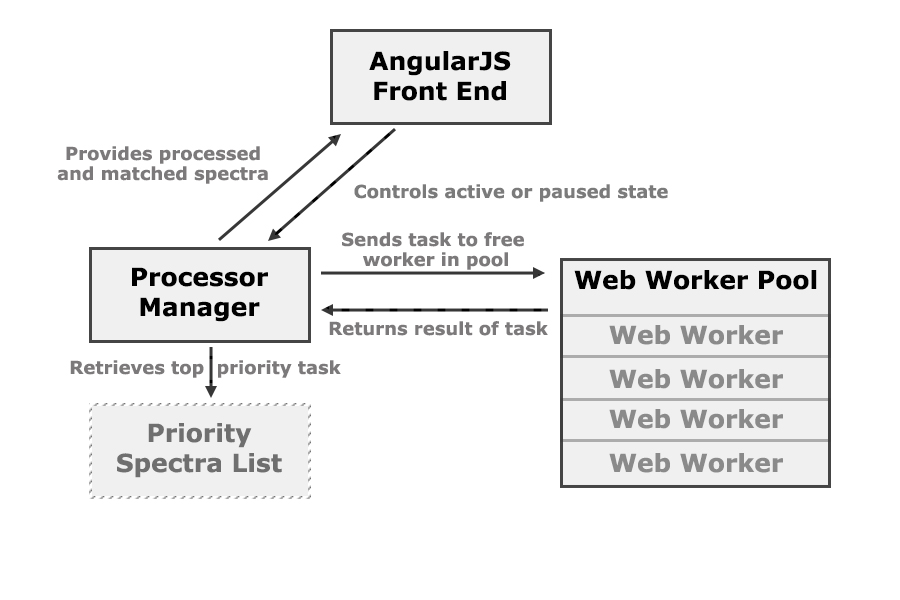
\includegraphics[width=0.8\textwidth]{images/diagram.jpg} 
\centering
\caption{A basic diagram showing the program structure, with arrows indicating interactions between components. It should be noted that communication with web workers is strictly done via native javascript objects, and as such both the data given to web workers and the results they send back is converted into a JSON string format to allow easy serialisation of more complicated data structures. The number of web workers displayed in the diagram is not representative of the program itself, which aims to have a minimum of one web worker, with the desired number being one less than the number of logical processors on the client system, ensuring that one processor is free if possible to handle the user interface, where in the case of a single core machine it is unavoidable for both the interface and analysis threads to be handled by the same processor.}
\label{fig:diagram}
\end{figure}



\section{User Interface}

\subsection{Landing Page}

The user interface developed initially leads users to an empty overview screen, with only the navigation menu and the side bar displaying, as is shown in Figure \ref{fig:empty}. This page has been kept empty so that the drag and drop prompt in the upper left hand corner of the screen will be located by the user in a minimum amount of time. From this page, a user can either navigate to other tabs, or drop a FITs file or a previously saved results file into the drop zone in the upper left hand corner of the page. With no other content to distract users, no one in user testing had difficulty dropping a file in as the first step of using the program. Some users did decide to navigate to the Usage page first, however.

\begin{figure}[ht!]
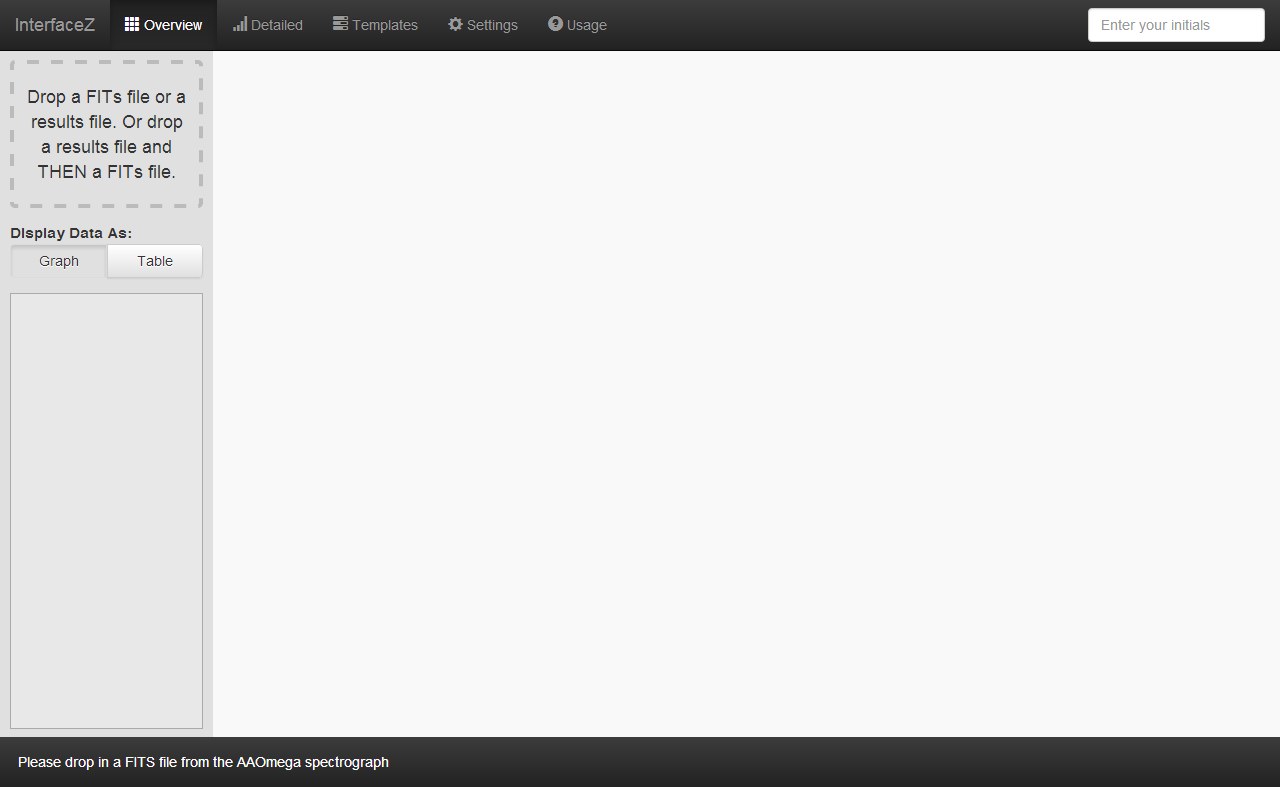
\includegraphics[width=1\textwidth]{images/empty.png} 
\centering
\caption{The landing page displayed to a user when they navigate to the site.}
\label{fig:empty}
\end{figure}



\subsection{Usage Page}

The Usage page serves as the programs Help page and menu, and can be accessed via clicking on the navigation menu or by pressing the ``?" key. The introductory segment, displayed in Figure \ref{fig:usage}, informs the user on the input expected by the program, how to load that input into the program, and then how to analyse it. It also details the automatic saving of results so the user knows closing the browser will not lose work, and provides contact links to the developer and issue tracking page so that any bugs or feature requests can be communicated easily.


\begin{figure}[ht!]
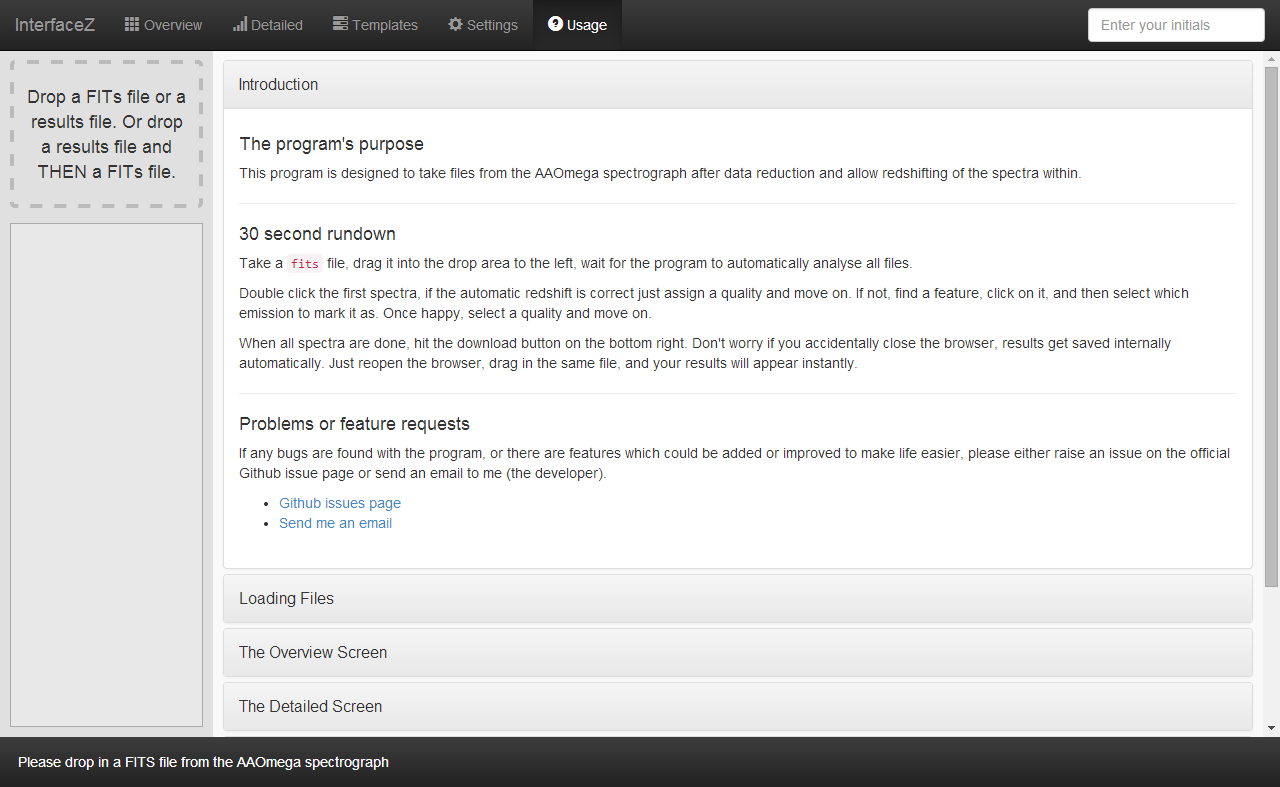
\includegraphics[width=1\textwidth]{images/usage.png} 
\centering
\caption{The usage page, with the introductory accordion expanded and all others collapsed.}
\label{fig:usage}
\end{figure}


The ``Loading Files" accordion section details reiterates how to load files in, and provides four compatible FITs files that are publicly hosted which can be downloaded and then given to the application if the user simply wants to use the application without having a data file of their own. This page also details the background processes that occur after dropping a file in: namely that each spectrum first gets preprocessed and then gets a redshift estimate given to users. This section explains that a progress bar will appear in the footer once a FITs file is dragged in, and that the progress through preprocessing is shown as a green progress bar, the progress through redshifting matching is shown as a red progress bar, and once all spectrum have a redshift, the progress bar will turn blue.


The accordion sections for the Overview, Detailed, Templates and Settings screen explain their function and how to interact with them. For example, the Detailed section explains how the template matching works, how to cycle through the best automatic results, how to manually adjust the redshift, how to mark spectral lines and how to assign a quality to the final redshift. The final section, on keyboard shortcuts, provides the user with a list of shortcuts, where they are applicable, and what they do. A section of this screen can be seen in Figure \ref{fig:keyboard}.

\begin{figure}[ht!]
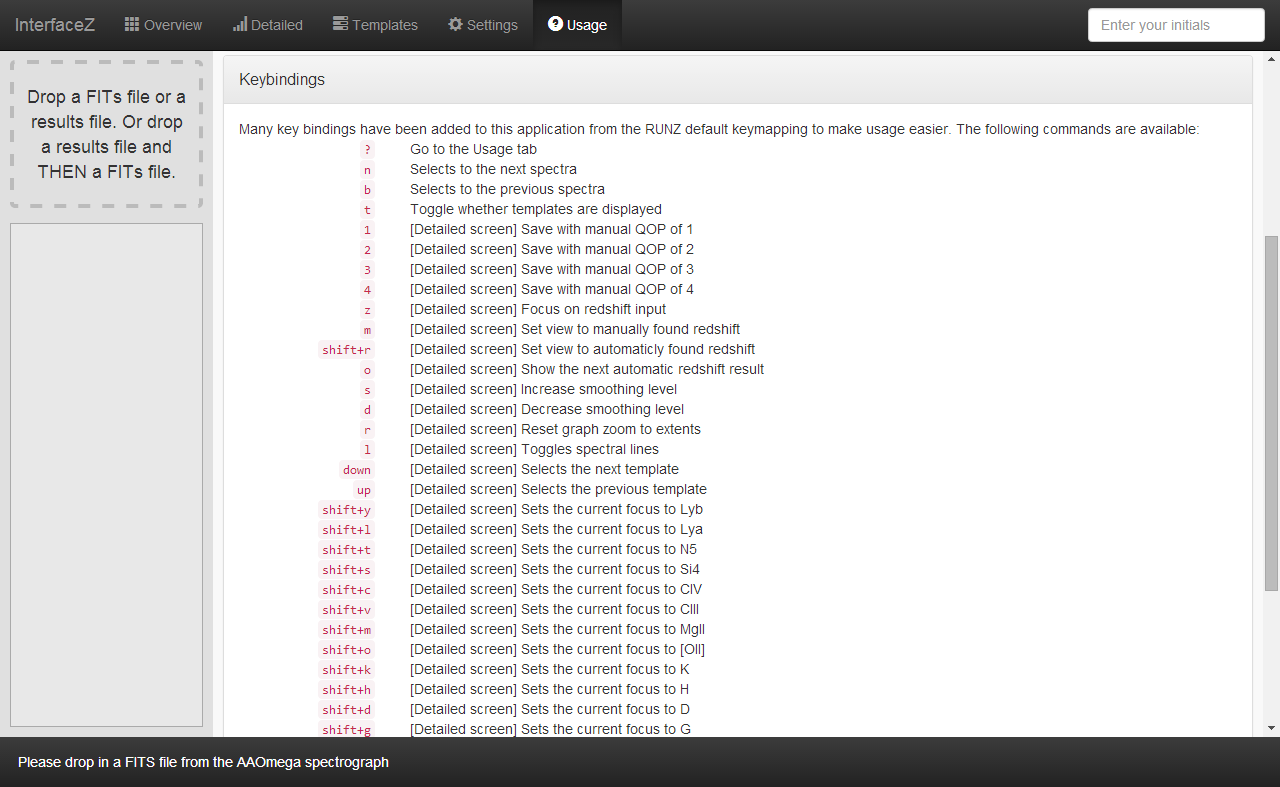
\includegraphics[width=1\textwidth]{images/keybindings.png} 
\centering
\caption{The keyboard shortcuts accordion presented to the user.}
\label{fig:keyboard}
\end{figure}


\pagebreak
\subsection{Overview Page}

After dragging and dropping a FITs file into the application, the Overview screen populates by default with a series of graphical tiles that show the spectrum in black and the currently matched template at the matched redshift in red. Figure \ref{fig:overviewGraph} shows this screen after preprocessing is complete and nine spectrum have been matched.

Whilst not specific to the Overview screen, notice that the drop zone has changed its display text to reflect the file which was given to the program, and the sidebar contains a more condensed list of spectrum with their redshift estimates and quality ratings that remains visible on any screen. As discussed in the Overview section, the progress bar visible in the page footer details how many spectrum have been analyses and how many are still remaining. The red colour of the progress bar in Figure \ref{fig:overviewGraph} indicates that the current state is redshift estimation, and the blue colour of the progress bar in Figure \ref{fig:overviewTable} indicates that all spectrum have had a redshift assigned. The user can pause and resume processing and matching via the Pause/Resume button in light blue in the footer, and can download the results of every spectrum that been assigned a redshift (via automatic matching or manual) when they click the ``Download" button to the right. The CSV file downloaded can be given to other users and its results loaded into the application via dragging and dropping onto the drop zone, or be used for database ingestion.

On both the graphical and tabular view, a user can select any spectrum by clicking on either the graph or the table row (for visual example, the first spectrum has been selected in Figure \ref{fig:overviewTable} as shown by the blue background of the first row), and a double click will take them to the detailed page with the selected spectrum set to the one they clicked on. In the tabular view, users can also reorder the results by clicking on the table headings, where a use case example of this sorting would be sorting by spectrum matching quality so that low quality spectrum can be reviewed.

The overview page has little extra functionality, as it mainly servers to present a large amount of coalesced data to the user rather than offer serious interactivity. 



\begin{figure}[ht!]
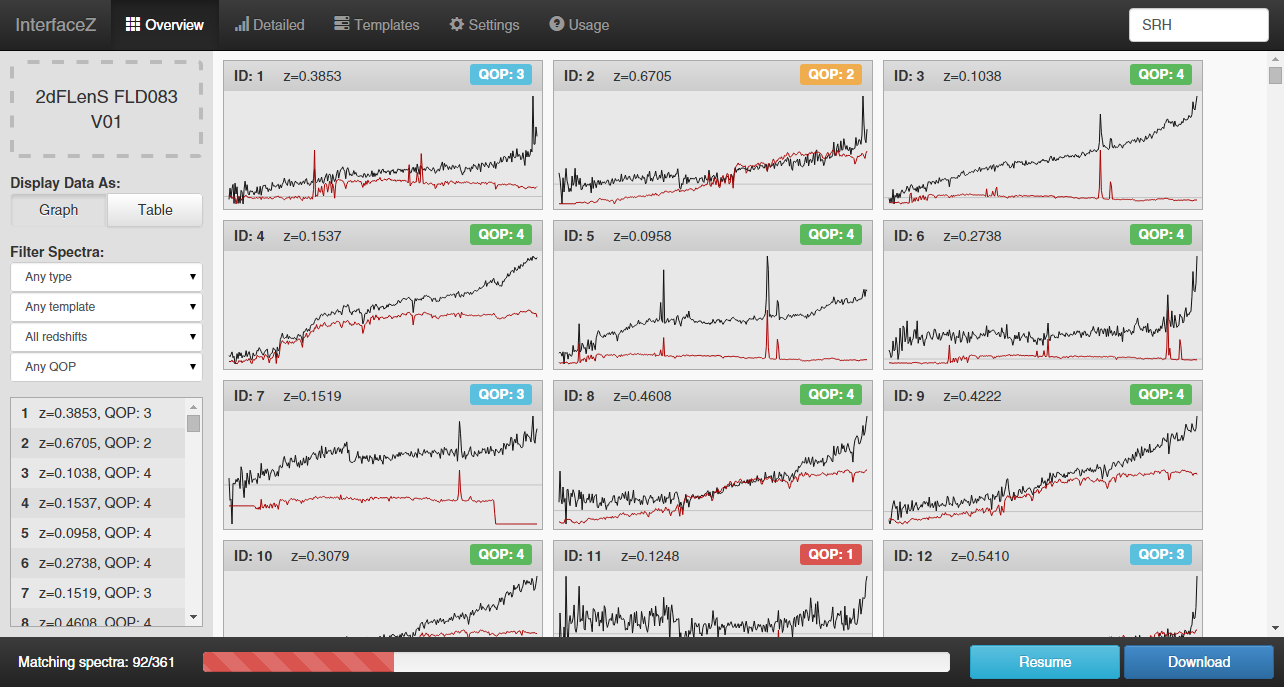
\includegraphics[width=1\textwidth]{images/overviewGraph.png} 
\centering
\caption{The Overview screen in graph mode, after dropping in a FITs file and letting the processing finish and the matching algorithm match nine spectrum.}
\label{fig:overviewGraph}
\end{figure}

\begin{figure}[ht!]
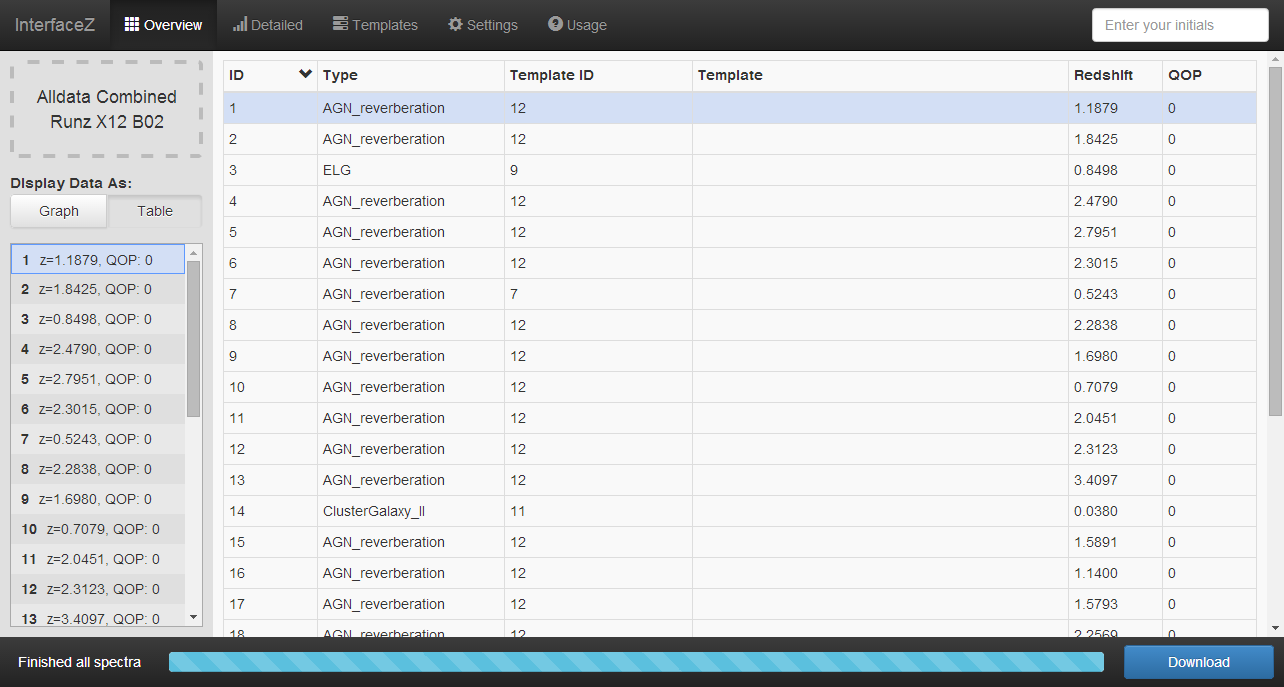
\includegraphics[width=1\textwidth]{images/overviewTable.png} 
\centering
\caption{The Overview screen in table mode, after dropping in a FITs file and letting the processing finish and the matching algorithm match all spectrum. The first row, corresponding to spectrum ID 1, is selected in this example.}
\label{fig:overviewTable}
\end{figure}





\subsection{Detailed Page}

The detailed page is where users review automatic redshifts and manually redshift any spectrum that were matched incorrectly by the automatic algorithm. Given the amount of features on the page, Figure \ref{fig:detailed} is supplied as a references, with the labelled UI elements and their functions described below.

\begin{figure}[ht!]
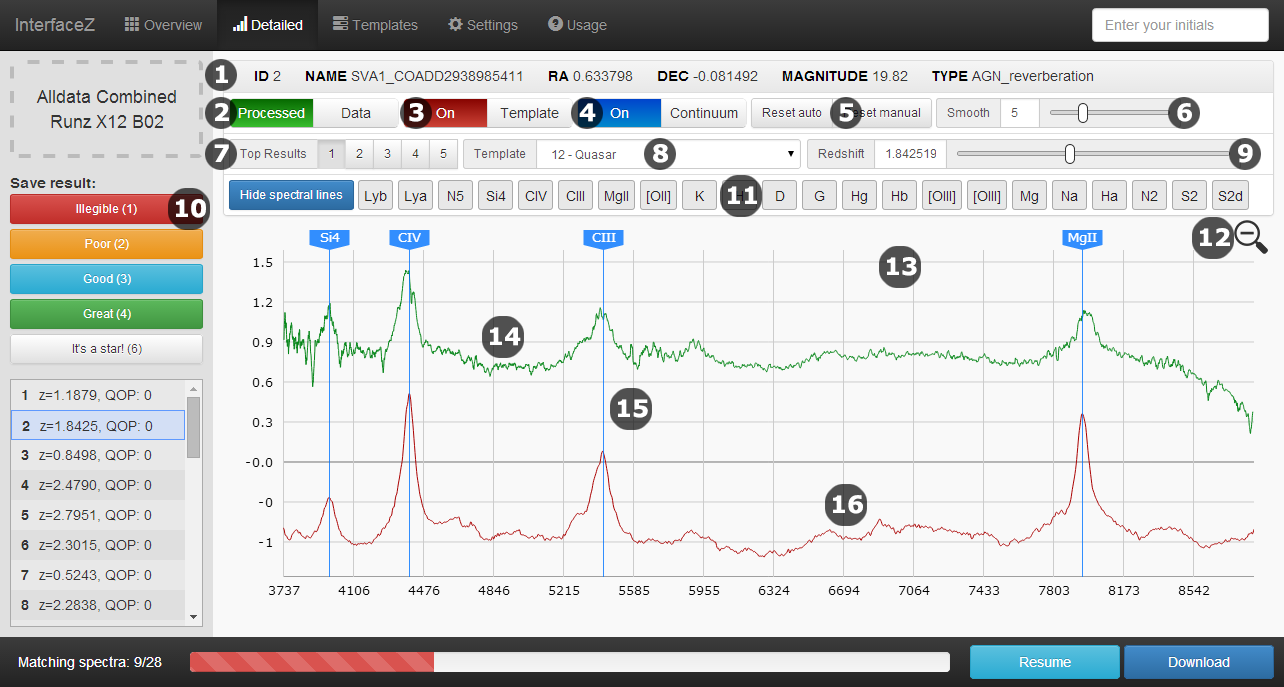
\includegraphics[width=1\textwidth]{images/detailed2.png} 
\centering
\caption{A labelled diagram of the detailed screen, with a quasar spectrum selected after automatic matching was completed for the spectrum.}
\label{fig:detailed}
\end{figure}

\textbf{Label Guide:}
\begin{enumerate}
\item \textbf{spectrum details header:} This header contains the spectrum ID, its name, right ascension, declination, magnitude and expected type.
\item \textbf{Data toggle:} With this toggle, a user can go from toggle between viewing raw spectrum data or the processed data. Processed data includes removal of blanks and detection of cosmic rays and a more advanced and computationally expensive continuum removal process.
\item \textbf{Template Toggle:} A user can click on this button to toggle the template either on or off. Most use cases involve the template being displayed, but in some circumstances the user may want to remove all non-spectrum data from the plot, and thus this toggle button is provided.
\item \textbf{Continuum toggle:} This toggle allows users to view spectrum and templates with or without continuum. Continuum subtraction algorithms are detailed in section \ref{sec:continuum}.
\item \textbf{Reset buttons:} The user is provided with two buttons, one to reset the template and redshift to the automatic match, and another to reset it to the manual match. In many cases where automatic matching is correct, these two options will be identical.
\item \textbf{Smoothing:} This slider allows users to smooth spectrum via boxcar smoothing where the smoothing number controls with window size applied in the smoothing process.
\item \textbf{Top Results:} After automatic matching has processed the selected spectrum, the top five automatic results are given to the user. These results can be viewed by simply clicking on the five numbered radio buttons.
\item \textbf{Template Selector:} This options input allows users to select a template from the twelve predefined templates or to select none at all. Changing templates does not change the previously selected redshift.
\item \textbf{Redshift:} Users can type in a desired redshift or drag the slider to scroll through values, where the redshift of the template displayed will instantaneously update to match the input redshift value.
\item \textbf{Quality Selectors:} By clicking on one of the five vertical buttons, users can save the currently selected template and redshift to a manual result with a given quality. Due to the target objects of the OzDES survey (extra-galactic), users can also mark spectrum as stars, so that they can be removed from consideration.
\item \textbf{spectral Lines:} A large part of manual matching is to mark spectral lines. This can be done by selecting a point on the graph, and then clicking on one of the available spectral lines. The line will be marked at the location selected, and the redshift determined from the marked wavelength with respect to the rest frame wavelength of the spectral line.
\item \textbf{Zoom Out:} As users can zoom into parts of the graph via clicking and dragging a window, this button allows users to zoom out to see the entire spectrum again.
\item \textbf{Graph Canvas:} The rest of the page area is given to canvas space. At the top of the canvas, any visible spectrum lines are marked, and a fixed pixel width grid is displayed to the user.
\item \textbf{spectrum Plot:} The top plot shown is the observed spectrum currently with a smoothing window of five pixels. Four broad quasar peaks are clearly visible in this spectrum.
\item \textbf{spectral Line Markers:} By default, all spectral lines are shown to the user, although they can be hidden via a ``Hide spectral lines" button (a blue button directly to the right of the the number 10 label). Line positions are determined via the current redshift, and scrolling through redshift details will therefore also scroll the positions of these lines, making it easier to match features.
\item \textbf{Template Plot:} The template plot is shown in red. The currently selected template is a quasar at redshift approximately 1.84, as shown in the template and redshift inputs (labels 8 and 9 respectively).
\end{enumerate}

The visual detail presented to the user at any time, and the instantaneous response of the user interface to all changes in input values is designed to minimise the amount of time taken for a user to select an accurate redshift, and increase the accuracy of the user's redshift estimates. In addition to the selectable elements detailed above, keyboard shortcuts using the same keys as the \runz{} application also work in the detailed page, making the transition process from \runz{} to the new software as easy as possible.

\pagebreak
\subsection{Templates Page}

The templates page is not actively used in redshifting spectrum, and serves to provide a graphical list of all templates to the user, with the wavelength range explicitly stated. 


\begin{figure}[ht!]
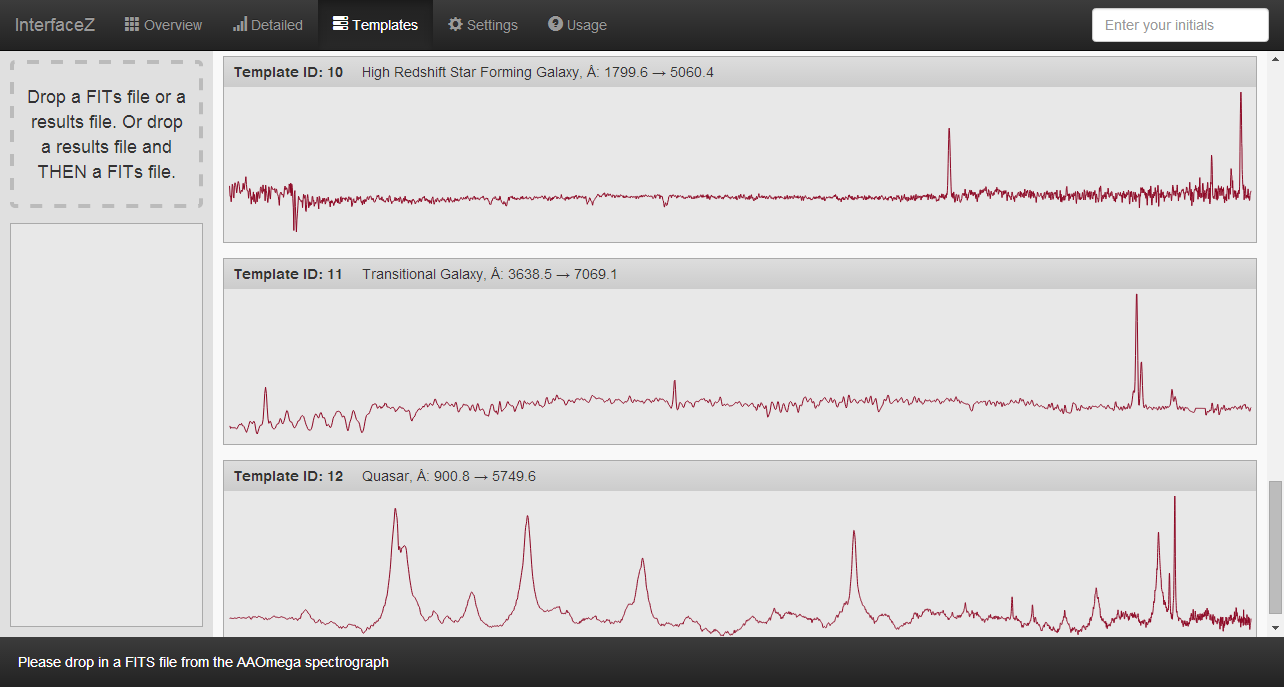
\includegraphics[width=1\textwidth]{images/templates.png} 
\centering
\caption{The templates screen, showing the last three templates in the catalogue: A high redshift star forming galaxy, a transitional galaxy and a quasar. This screen is most useful when customising the template catalogue, and standard redshifting use cases do not have users visiting this screen in the redshifting process.}
\label{fig:templates}
\end{figure}



\subsection{Settings Page}

The settings page is also a page outside of usage for the redshifting process. It's primary functionality that it is used for is to override the number of processors being used by the application, and to delete previously determined results. The former scenario is useful in the case where the user interface starts to slow due to intense background processing, and the latter is useful when an update to the matching algorithm may warrant re-redshifting spectrum, requiring the past results to be cleared from the system. Results can be deleted globally for all input FITs files, or they can be deleted for a FITs file when loaded in (to preserve the matching results for other files). Settings on this page persist between user settings and are stored as site cookies, and any settings changed apply instantly and can be reversed. As deleting saved results cannot be reversed, a cautionary banner is displayed at the top of the settings page, and a confirmation dialogue box is displayed to the user when attempting to clear any saves.


\begin{figure}[ht!]
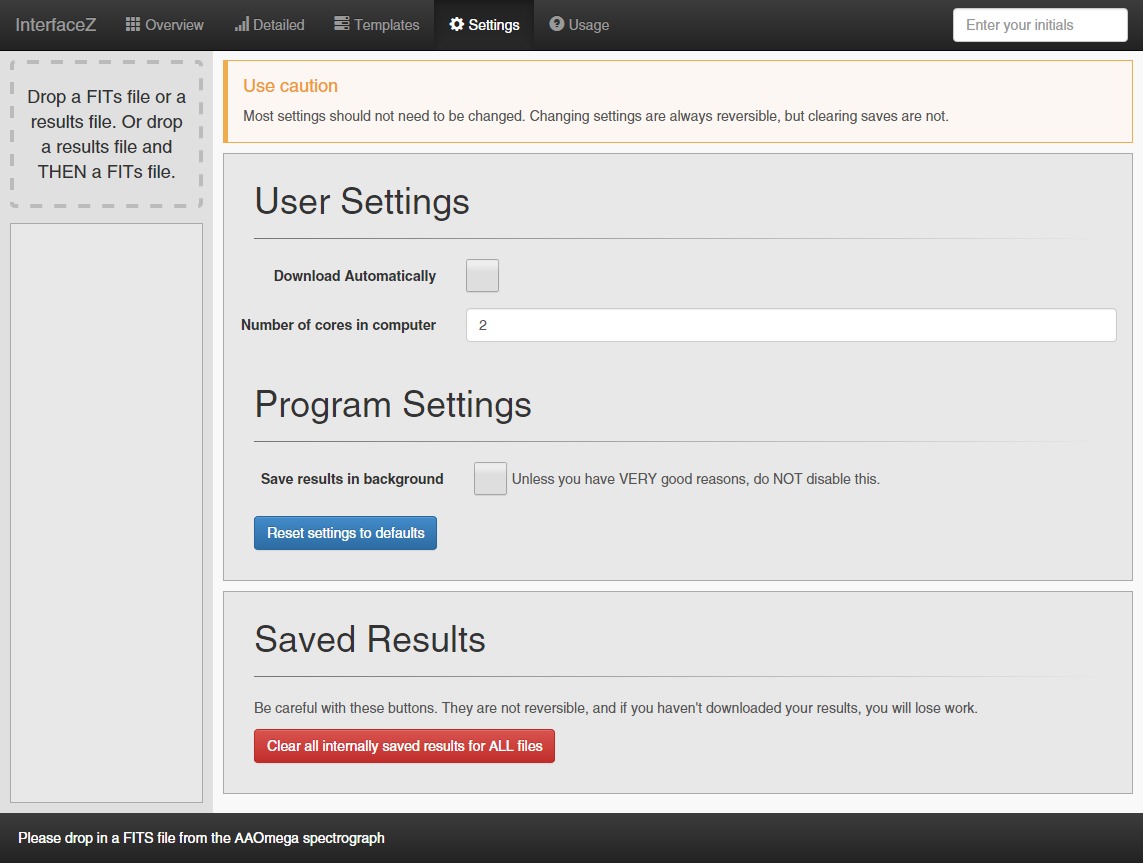
\includegraphics[width=1\textwidth]{images/settings.png} 
\centering
\caption{The full settings page, with the few settings that are currently available to users.}
\label{fig:settings}
\end{figure}


























\pagebreak
\section{Processing algorithm}

The processing algorithm is responsible for presenting the end user with a visual representation of a spectrum to manually redshift as quickly as possible, with defects such as blanks and cosmic rays automatically removed, and to have the spectrum available with and without continuum. Many steps in the processing and matching algorithms are based of the algorithms written by Ivan Baldry \cite{baldry2014galaxy}. Each spectrum contains two data arrays, containing the intensity (amplitude) values and variance respectively.

\subsection{Removing Bad Pixels}

A pixel is determined to be bad if it satisfies any of a number of criteria, which are as follows: if the spectrum intensity or variance is not a number or is null, if the variance is negative, or if the spectrum intensity is greater or less than specific thresholds. If a pixel matches those criteria, it's intensity and variance is replaced with a mean over a window before and after pixel where only good pixels in the window are considered in the average.

This process can be described mathematically via the following formula, where $s_i$ represents the $i$th element of the spectrum intensity, $v_i$ represents the $i$th element of the spectrum variance, and $n$ is the floored half window width, such that a window of nine pixels (value currently in use) would give $n=4$.
\begin{align}
s_i &= 
\begin{cases}
	\brac{\sum\limits_{j=i-n}^{i+n} \begin{cases}1 & \text{if } \lnot f(j) \\ 0 & \text{otherwise} \end{cases}}^{-1}\brac{\sum\limits_{j=i-n}^{i+n} \begin{cases}s_j & \text{if } \lnot f(j) \\ 0 & \text{otherwise} \end{cases}} & \text{if } f(i) \\
	s_i & \text{otherwise}
\end{cases}\\
\text{such that } f(i) &= \brac{s_i > 10^6} \vee \brac{s_i <  -\left(10^4\right)} \vee \brac{v_i < 0} \vee \brac{s_i \notin \mathbb{R}} \vee \brac{v_i \notin \mathbb{R}}.
\end{align} 

Whilst the equation above deals with the spectrum amplitude $s_i$, an identical procedure is followed for the variance as well.

\pagebreak
\subsection{Removing Cosmic Rays}

Cosmic rays are detected via flagging points more than thirty standard deviations from the mean and the maximum neighbouring point. Points that satisfy these criteria are replaced with a average intensity over a window to either side such that only points less than thirty standard deviations from the mean are considered part of the average. The variance for these points is set to a maximal value, currently set as $10^{10}$, which has the effect of marginalising the pixel contribution to cross correlation when it is eventually performed. The window size for averaging is set to five, such that $n = 2$.

\begin{align}
s_i &= 
\begin{cases}
	\brac{\sum\limits_{j=i-n}^{i+n} \begin{cases}1 & \text{if } \lnot f(j) \\ 0 & \text{otherwise} \end{cases}}^{-1}\brac{\sum\limits_{j=i-n}^{i+n} \begin{cases}s_j & \text{if } \lnot f(j) \\ 0 & \text{otherwise} \end{cases}} & \text{if } f(i)\land g(i) \\
	s_i & \text{otherwise}
\end{cases}\\
v_i &= 
\begin{cases}
	10^{10} & \text{if } f(i)\land g(i) \\
	v_i & \text{otherwise}
\end{cases}\\
\text{such that } f(i) &= \brac{\abs{s_i - \mean{s_i}} > 30 \sigma}, \\
\text{and } g(i) &= \brac{max\brac{\abs{s_i - s_{i-1}}, \abs{s_i - s_{i+1}}} > 30 \sigma}.
\end{align} 


\subsection{Removing Continuum} \label{sec:continuum}

Continuum is subtracted from the spectrum via the means of rejected polynomial fitting. A six degree polynomical is fitted to the spectrum, and any points more than 3.5 standard deviations from the fitted polynomial are removed from consideration. A new polynomial is fitted to the remaining points, and points greater than 3.5 standard deviations are again rejected. Iterations stop after a maximum number of fifteen iterations or until all points are within 3.5 standard deviations of the polynomial. The rejections serve the purpose of conforming the polynomial to the actual continuum so that no warping of the fit occurs to try and match strong features and emission lines.



\section{Matching algorithm}

After removing bad pixels, cosmic rays and continuum subtraction, the spectrum is duplicated, one to undergo quasar matching, and the other to match other templates, referred to as the generic and quasar spectrum respectively. The generic spectrum is used to match the group of non-quasar templates, and the quasar spectrum is used only to match the quasar template.

\subsection{Further preprocessing}

Further continuum subtraction applies to only the generic spectrum. This second step of continuum subtraction generates a median filter of width 51 pixels (25 pixels to either side of the target pixel) and then applies boxcar smoothing of 121 pixels onto the generate median filter results, where a typical AAOmega spectrum is comprised of 4941 pixels. The result of the boxcar smoothing is subtracted from the spectrum intensity to further remove continuum. This step is not applied to the quasar template as the broad peaks of the quasar template get subtracted out. Figure \ref{fig:smooth} shows the spectra intensity before and after subtraction, with the median filter with and without smoothing also illustrated.\\
\begin{figure}[ht!]
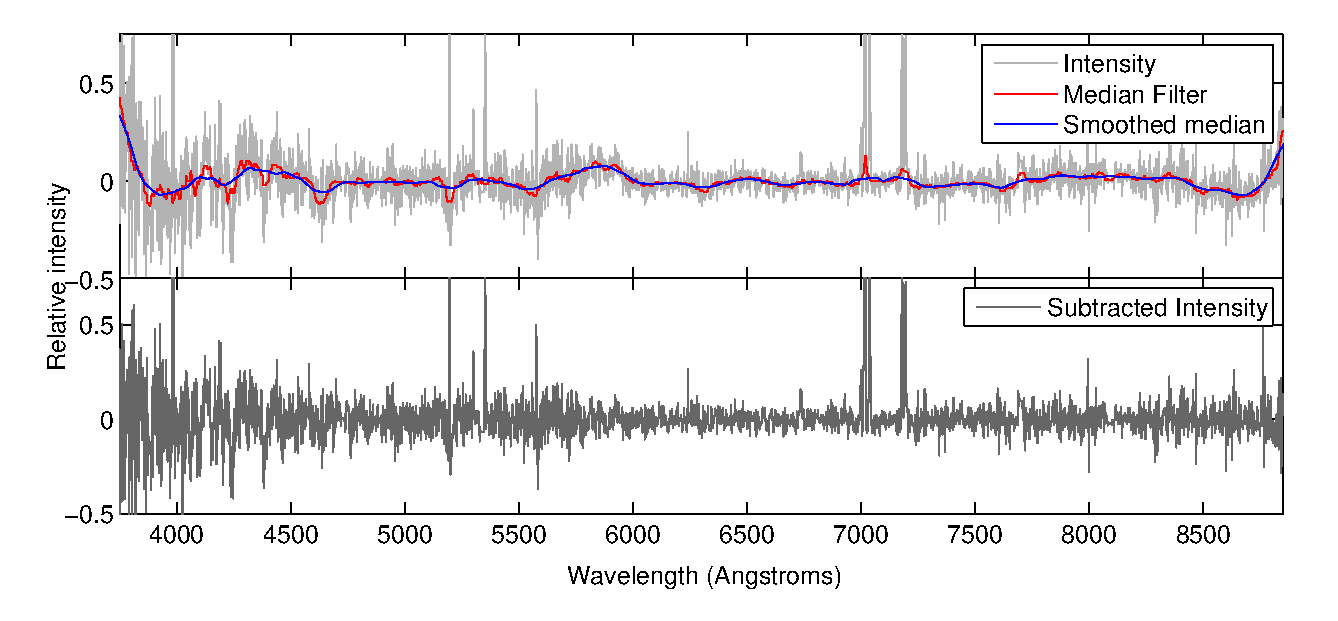
\includegraphics[width=\textwidth]{images/smoothing.eps} 
\centering
\caption{The final process of continuum subtraction is shown, with the smoothed median filter to be subtracted shown in the top subplot.}
\label{fig:smooth}
\end{figure}


The quasar template, instead of having the second step of continuum subtraction applied, instead smooths the spectrum. In order to smooth out broad features but preserve pixel peak location, a seven pixel window decaying mean filter is applied with a decay factor of 0.9. As the generic spectrum matches on narrow emission and absorption features, it would negatively impact matching performance to smooth those features, unlike the broad quasar features. Formally, for each point in the quasar spectrum $s_i$, 

\begin{align}
s_i = \frac{\sum\limits_{j = i -n}^{i+n} \beta^{\abs{j-i}} s_j}{\sum\limits_{\alpha=-n}^n \beta^{\abs{\alpha}}},
\end{align}
where a window size of seven pixels gives $n=3$ and the decay factor gives $\beta = 0.9$. The quasar spectrum before and after this process is shown in Figure \ref{fig:quasar}.

\begin{figure}[ht!]
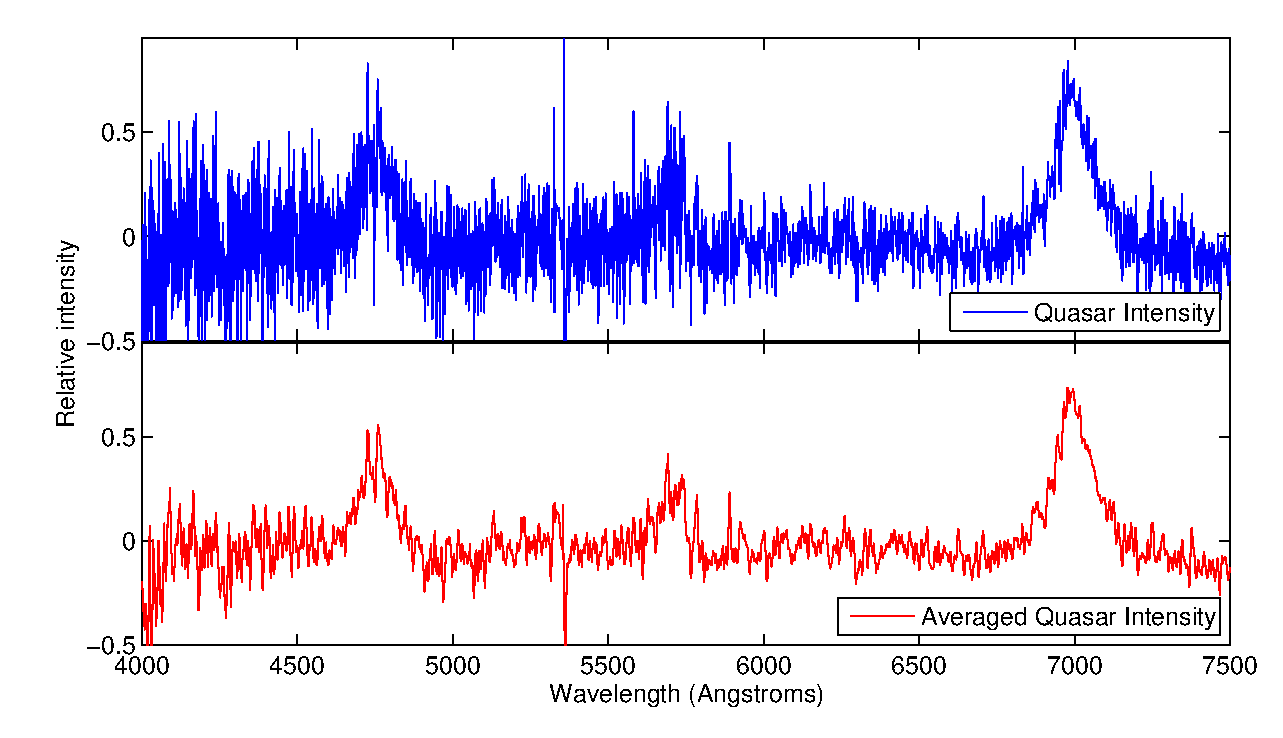
\includegraphics[width=1\textwidth]{images/quasarAverage.eps} 
\centering
\caption{Smoothing of the quasar spectrum via application of a decaying mean filter.}
\label{fig:quasar}
\end{figure}


Finally, both the generic and quasar spectrum undergo tapering (also known as a window function or apodization), which is required to remove ringing from a Fourier transform  of the signal and smooth discontinuities. The transformation of the spectrum is discussed in section \ref{sec:transform}. Tapering is achieved via a sixty pixel sinusoid taper with five pixels of zero padding. The front taper can be described thus:


\begin{align}
s_i &= 
\begin{cases}
	0 & \text{if } i < p \\
	s_i \sin\brac{\frac{\pi (i-p)}{2w}} & \text{if } i < (p+w) \\
	s_i & \text{otherwise},
\end{cases}
\end{align} 

where $p$ represents the zero padding width ($p=5$), and $w$ represents the taper width ($w=60$).

\subsection{Error Adjustment}

Variance modification is only applied to the generic templates, and involves three steps: broadening variance, median adjustment and division of the spectrum by the variance squared. To account of subpixel differences in sky subtraction, variance is first broadened over adjacent neighbour pixels, such that for all point in the variance spectrum $v_i$, 

\begin{align}
v_i = \mathrm{max}(v_{i-1}, v_i, v_{i+1}).
\end{align}

After this, to remove pixels that have variance far below their neighbours, the error for each point is adjusted to be the maximum between the current value, and 0.7 times the median of a 13 pixel window centred around the pixel in question, such that

\begin{align}
v_i = \mathrm{max}\brac{v_i, 0.7\cdot \median\{v_{i-n}:v_{i+n}\}}.
\end{align}

After this variance adjustment, I divided the intensity spectrum by the variance spectrum squared as justified by Saunders \etal \cite{saunders2004improvements} in order to down-weight pixels with greater variance, such that for all $s_i,\ s_i = s_i \cdot v_i^{-2}$.

This step was not implemented on the quasar template, as the variance in the error spectrum meant that diving by the variance squared polluted the broad peaks to such an extent that they were unmatchable. Instead, the quasar spectrum does not consider spectrum error, as the broadness of the peaks means that individual uncertainty on a pixel basis is unimportant to the final result.

\subsection{Normalisation and Cross Correlation} \label{sec:transform}

Both the generic and quasar spectrum undergo RMS normalisation such that $s_i = s_i \sigma^{-1}$ before undergoing cross correlation. Both spectrum are then oversampled and rebinned in an equispaced logarithmic array of $32\;768$ elements from the range $10^{2.8}$ to $10^{4.3}$, where those exponent values are chosen to allow for the full redshift range for each template. Both spectrum are then Fourier transformed into the frequency domain.

The template catalogue, upon program initialisation, also undergoes the preprocessing described in previous sections (where the quasar template takes the place of the quasar spectrum, and all other templates take the place of the generic spectrum), and they are rebinned as well, transformed in the frequency domain, and the complex result is conjugated.

The transformed generic spectrum is then multiplied with the non-quasar transformed templates, inverse transformed, circularly shifted half the size of the inverse array length and a subsection of the results are returned, where the subsection is determined by the allowed redshift ranges of each specific template. These results of this selection then have a rejected mean subtracted, where the mean is defined as the average value of all but the greatest 4\% of points. The subtracted values are then are normalised using their RMS value, just as the original intensity spectrum was normalised before Fourier transformation.

\subsection{Peak Selection}

The normalised cross correlation data then undergoes peak selection, in which peaks are identified over a five pixel window, such that for the cross correlation values $c_i$, an index $i$ is identified as a peak if it was greater than its four nearest neighbours (2 pixels to either side), formally defined as satisfying the criteria of

\begin{align}
\brac{c_i \geq c_{i+1}} \land \brac{c_i \geq c_{i+2}} \land \brac{c_i > c_{i-1}} \land \brac{c_i > c_{i-2}}.
\end{align}

Cross correlation peaks then had a quadratic fitted over that 5 pixel window, and the maximum value of the fitted quadratic, along with its effective index, is set to as the detected peak. Given that the domain after inverse transformation is in the original wavelength domain, a peak at index $i$ from the centre pixel represents a redshift of 

\begin{align}
z = \brac{10^{iN} (1+z_0)} - 1,
\end{align}

where $N$ is the Angstrom gap between adjacent pixels in the equispaced log scale and $z_0$ is the initial redshift of the provided template.

\subsection{Coalescing Peak Results}

Each of the templates generates a list of peak values, and these are required to be coalesced into a single output stream before being returned as the list of top results. The first step in this process is apply peak weighting, where the provided object type of the spectrum acts as a prior to the peak selection. Objects without prior assigned types are not weighted. These priors - the result of previous data gathering and photometric estimates, provide types that range from Supernova hosts, to Cluster Galaxies, Radio Galaxies, Emission Line Galaxies, Stars and Active Galactic Nuclei (quasars). Each template has a set of weights for each prior, and these weights are multiplied by the peak height in order to determine an adjusted peak strength.

After combining the weighted peak results for all templates into a singular list of peaks, the result is sorted, redshift values are rounded to five decimal places, and the best five results are return to the client interface thread, where they become visible to the user.

\textcolor{red}{NEED TO FINISH ACTUALLY DOING THIS. HAVE NOT DONE QUADRATIC FIT YET}

\section{Performance} \label{sec:performance}

The final performance of the matching algorithm is shown graphically in Figure \ref{fig:final}. Figure \ref{fig:final} and other similar figures throughout this document, unless otherwise specified, are created from by comparing manual redshift estimates with automatic redshift estimates from a collection of data files provided by Conor O'Neill and provides over a thousand different spectrum, with many spectrum available for more than one observation time (such that multiple observations of the same object are stacked to increase the signal to noise ratio). 

\textcolor{red}{ELABORATE ON THIS AFTER ACTUALLY FINALISING.}


\begin{figure}[ht!]
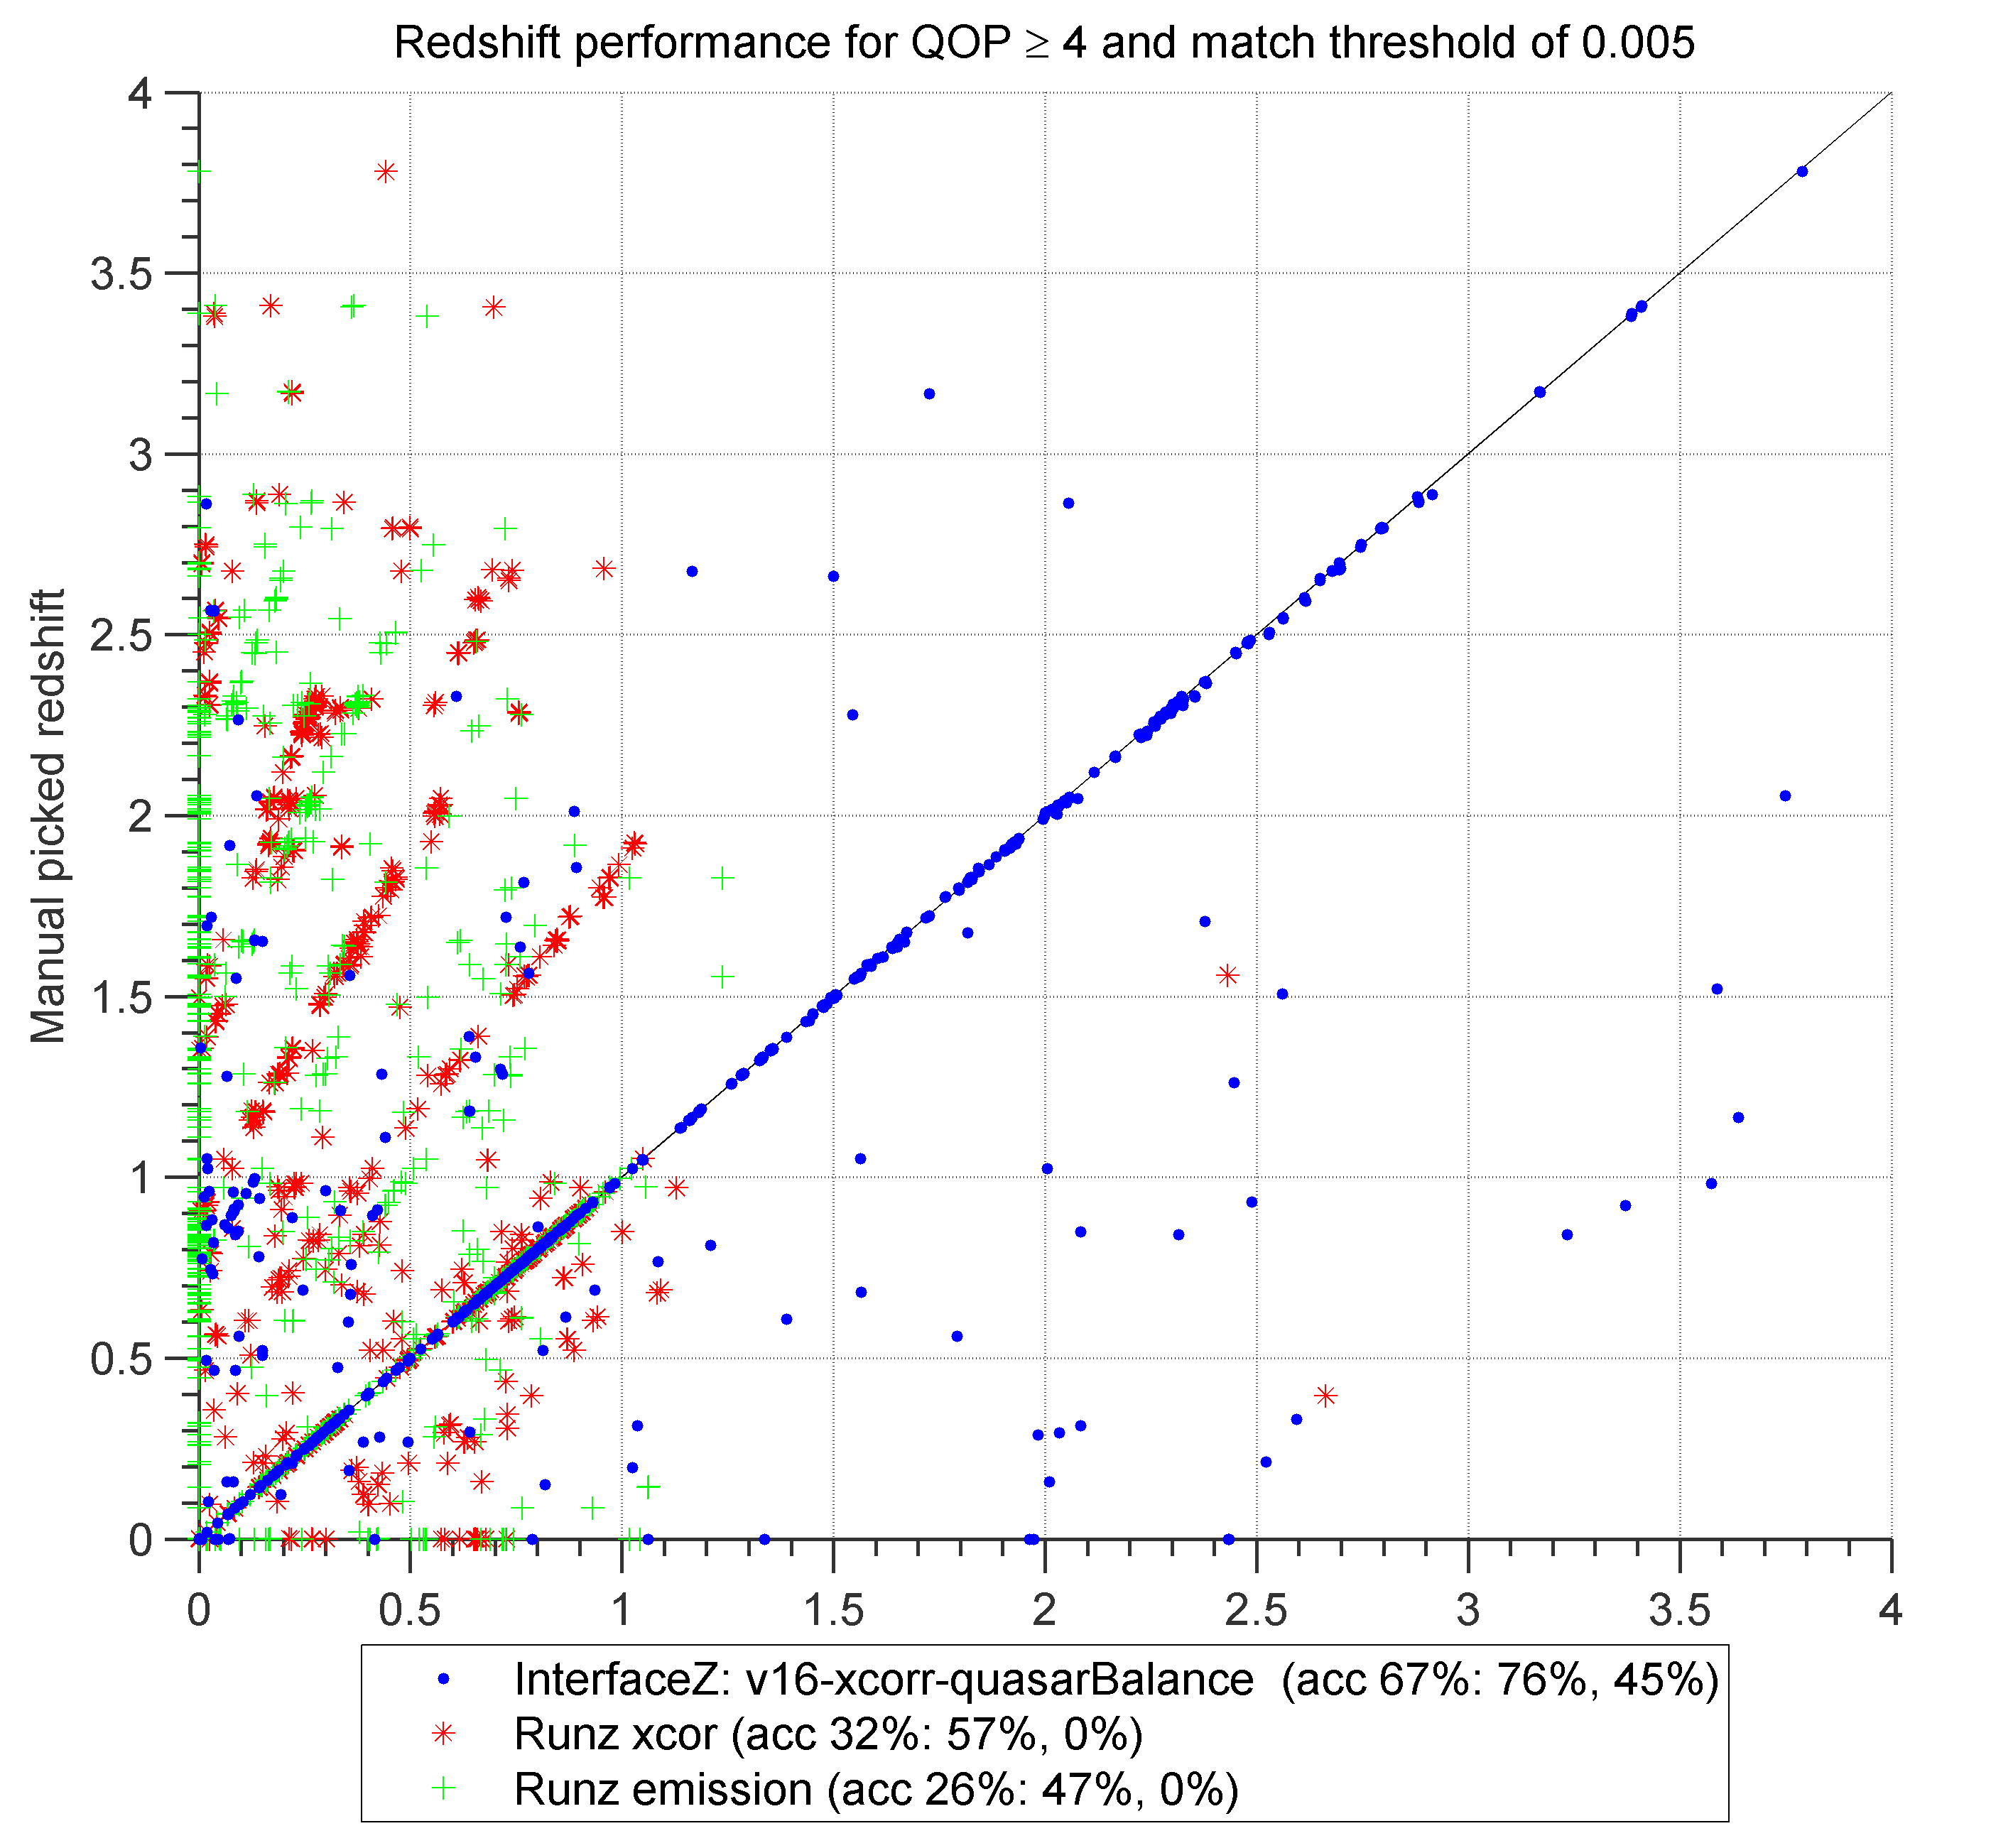
\includegraphics[width=0.8\textwidth]{images/final.png} 
\centering
\caption{Comparison of manual redshifts with automatically determined redshifts by the unweighted $\chi^2$ algorithm and by the two algorithms in use with \runz{}. The sixteenth iteration of matching algorithm is shown.}
\label{fig:final}
\end{figure}



\pagebreak
\section{Alternate Implementations}

A simpler matching algorithm was investigated during the early stages of this project, which utilised $\chi^2$ matching instead of cross correlation. This algorithm involved similar steps of continuum subtraction, but instead of cross correlating templates, each template had the $\chi^2$ difference calculated for a range of redshift values, such that 

\begin{align}
\chi^2_z = \sum\limits_i \brac{\frac{s_i - t_{iz}}{v_i}}^2,
\end{align}

where $s_i$ is the spectrum at index $i$, $t_i$ is the template at index $i$ after redshifting the template by value $z$ and $v_i$ is the error spectrum at index $i$. Performance of this implementation is discussed in \ref{sec:performance}, and my attempts to increase performance of the $\chi^2$ results to acceptable levels ultimately did not succeed to the extent where the cross correlation performance could be matched. A modified $\chi^2$ system was also investigated, such that 

\begin{align}
\chi^2_z = \sum\limits_i \brac{\frac{w_i\brac{s_i - t_{iz}}}{v_i}}^2,
\end{align}

where $w_i$ is a weight vector used to control the significance of specific pixels. Analysis was conducted with the weight vector set to the template intensity, the spectrum intensity, the square root of the spectrum intensity, and the product of the spectrum and template intensity, with minimal improvement in results.

The largest problem with the $\chi^2$ implementation was dealing with non-complete spectrum overlaps, an example of which is provided in Figure \ref{fig:overlap}. More formally, difficulty arose in how to include in the $\chi^2$ sum terms in which $t_{iz}$ did not exist. Not including the terms resulted in far lower $\chi^2$ terms for maximally shifted templates regardless of whether or not the maximal redshift values were a valid match or not. Commonly, the reduced $\chi^2$ is used to determine a goodness of fit \cite{Glover}, where $\chi_{\text{red}}^2 = \chi^2 / N$, where $N$ is the number of elements in the sum. However, this was still not an adequate solution as template normalisation before taking the $\chi^2$ difference was designed such that the template would be scaled to give the minimum $\chi^2$ result, and thus even the reduced $\chi^2$ for minimally overlapping spectrum continued to beat the $\chi^2$ result of the correct match for many spectrum.

\begin{figure}[ht!]
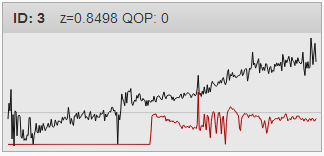
\includegraphics[width=0.5\textwidth]{images/overlap.png} 
\centering
\caption{An example match in which the template spectrum does not overlap the observed spectrum, with the spectrum shown only matching the template for approximately half of the spectrum pixels.}
\label{fig:overlap}
\end{figure}

The redshifts in which minimal overlap results in erroneous matches can clearly be seen as vertical lines in Figure \ref{fig:vertical}. The most promising method of reducing the goodness of fit of minimally overlapping spectrum was found to be in calculating a reduced $\chi^2$ using instead of the standard $r = N$, where $r$ is the reduction factor (where $N$ is the number of data points matched), a reduction factor of $r = \brac{\sum_{i=1}^N s_i}^{5/2}$ was used. This value simply represents the sum of all the spectrum points that were used in the $\chi^2$ calculation raised to the power of $5/2$. The power factor of $5/2$ has no rigorous theoretical foundation, it was simply found that squaring the sum of the weights provided insufficient disadvantage to minimal overlaps, and cubing the sum punished overlaps to a greater extent than desired such that no spectrum with any overlap would ever be returned as the best match. Comparison between Figures \ref{fig:vertical} and \ref{fig:novertical} show the decrease in vertical banding when the power of the weight sum was changed from $2$ to $5/2$.

\begin{figure}[ht!]
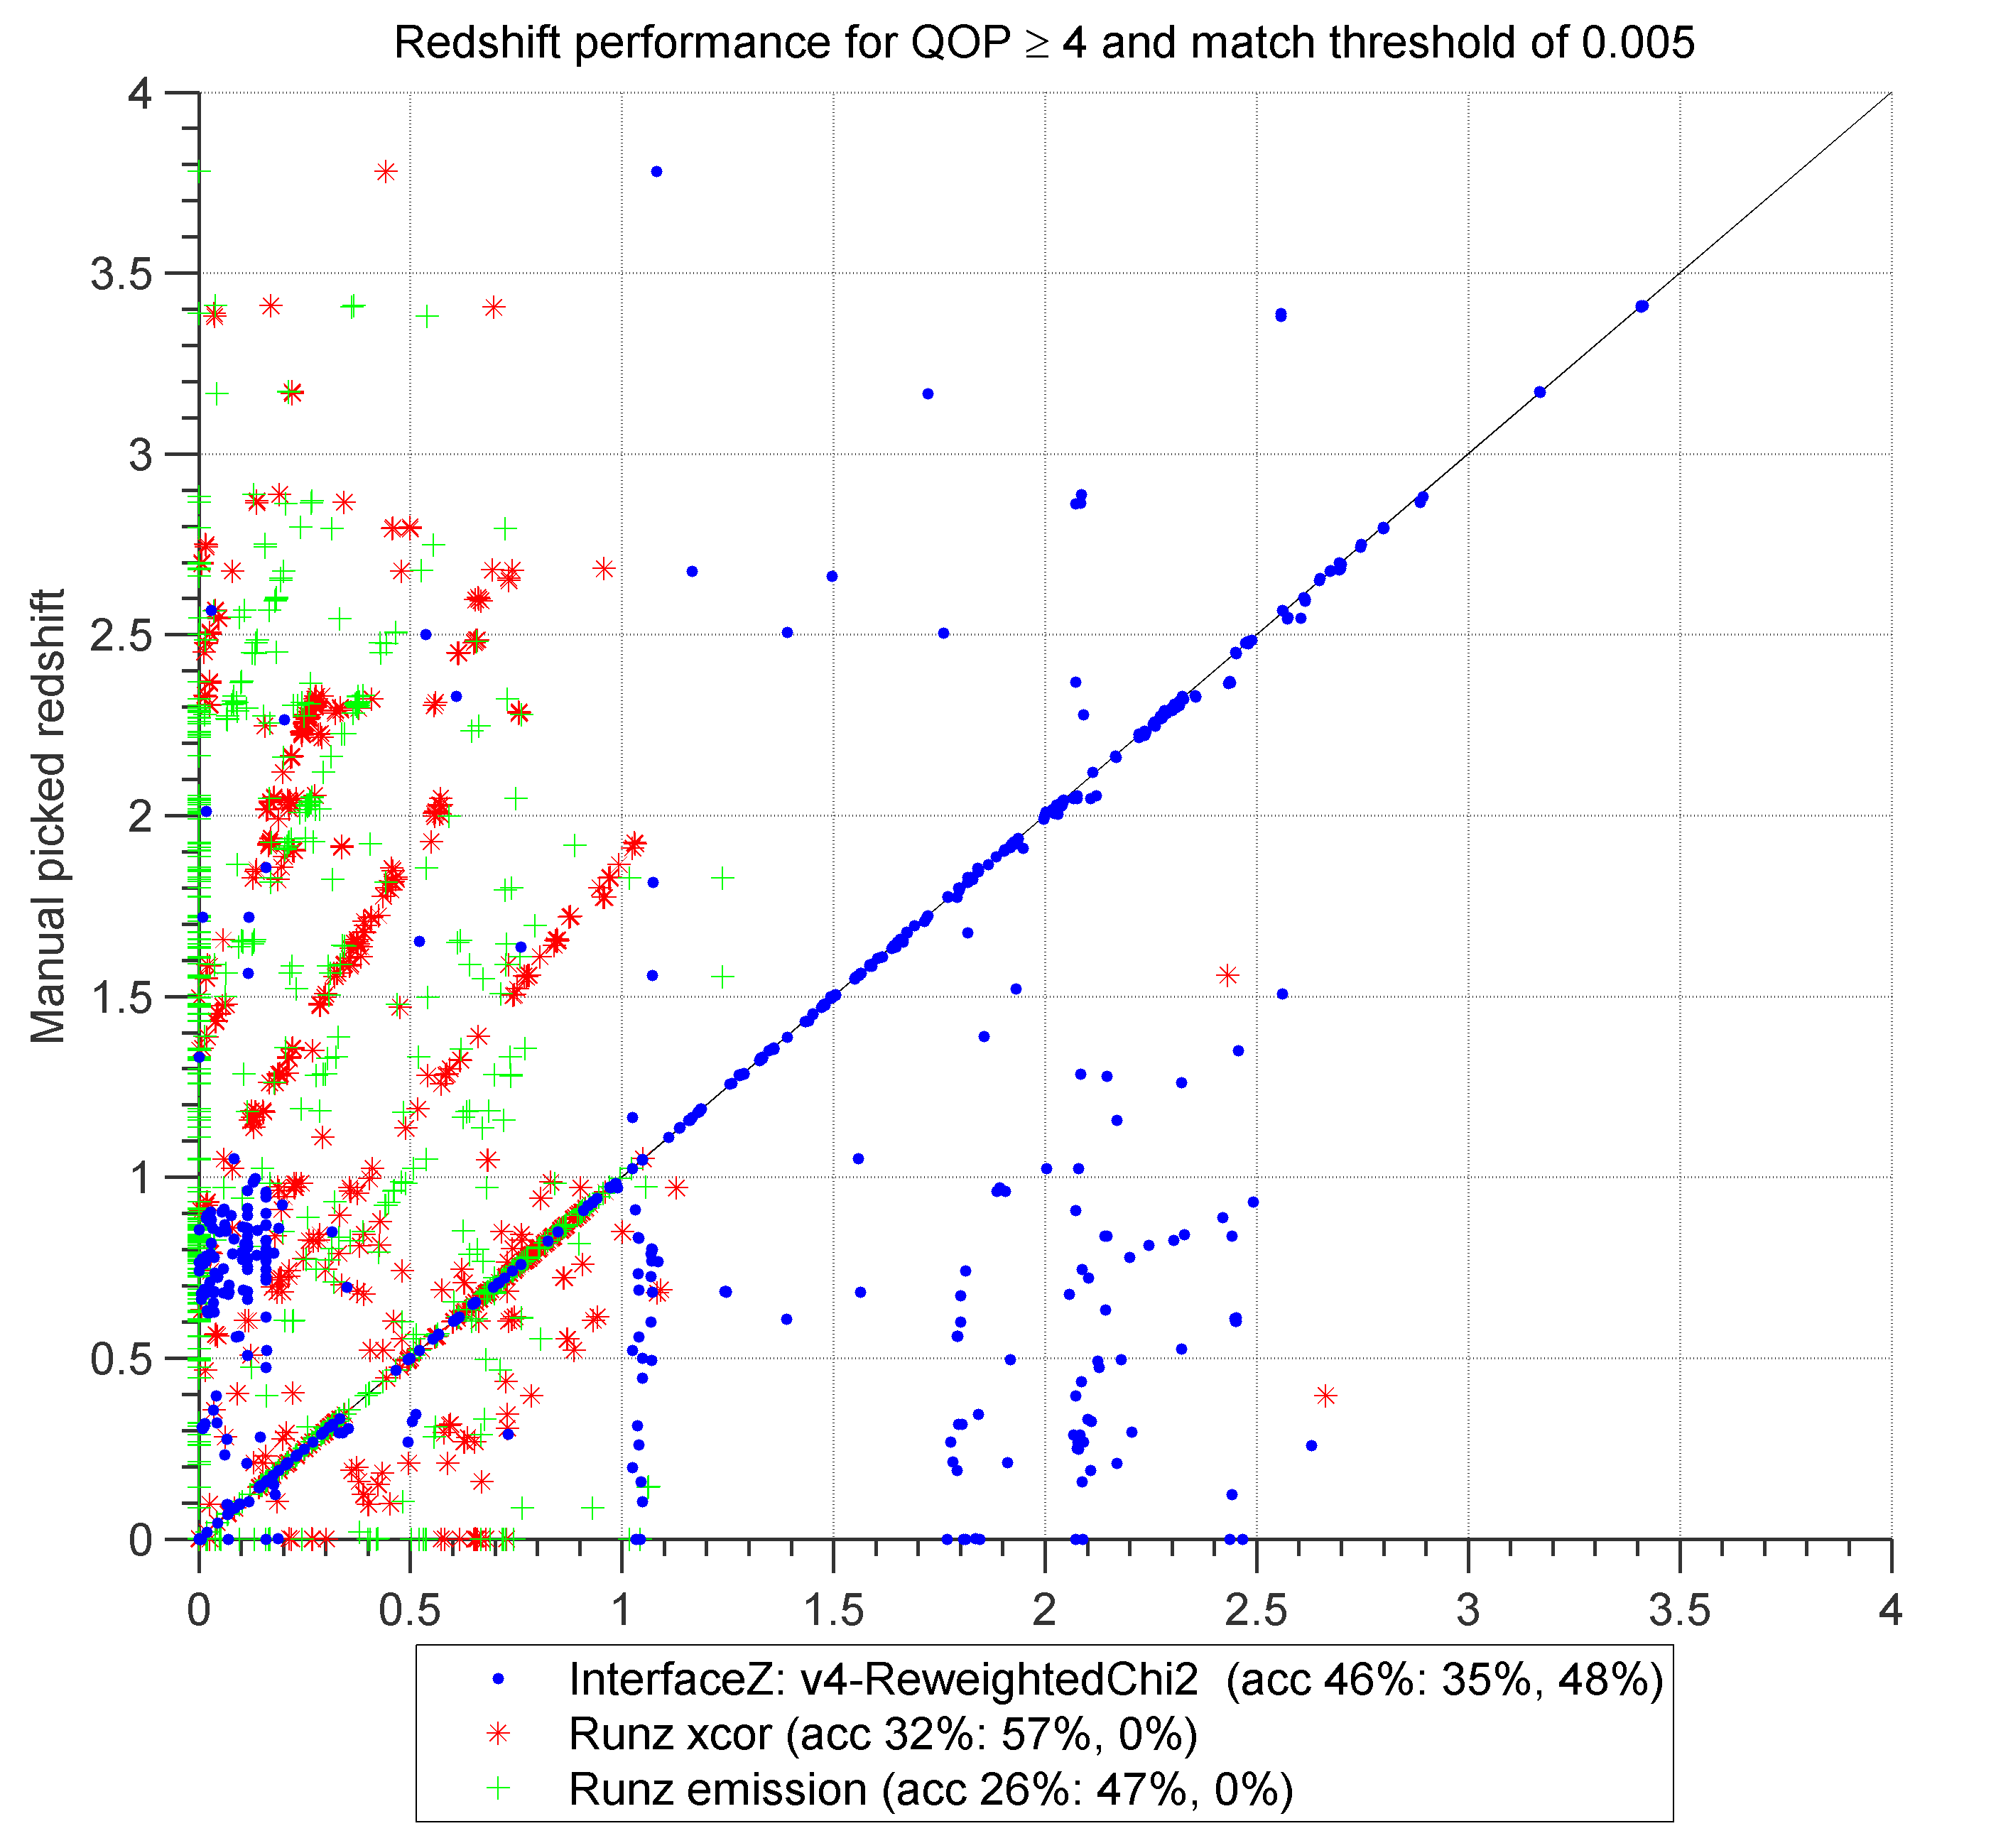
\includegraphics[width=0.9\textwidth]{images/Fullv4-ReweightedChi2.png} 
\centering
\caption{Comparison of manual redshifts with automatically determined redshifts by the unweighted $\chi^2$ algorithm and by the two algorithms in use with \runz{}. The fourth iteration of the reweighted $\chi^2$ matching algorithm is shown here, which used $w_i = \sqrt{\abs{s_i}}$ and $r = \brac{\sum_{i=1}^N s_i}^{2}$. Vertical result banding is found at redshifts in several places, most obviously the strong banding at approximately $z=1$, which corresponds to minimal overlap of galaxy templates.}
\label{fig:vertical}
\end{figure}

\begin{figure}[ht!]
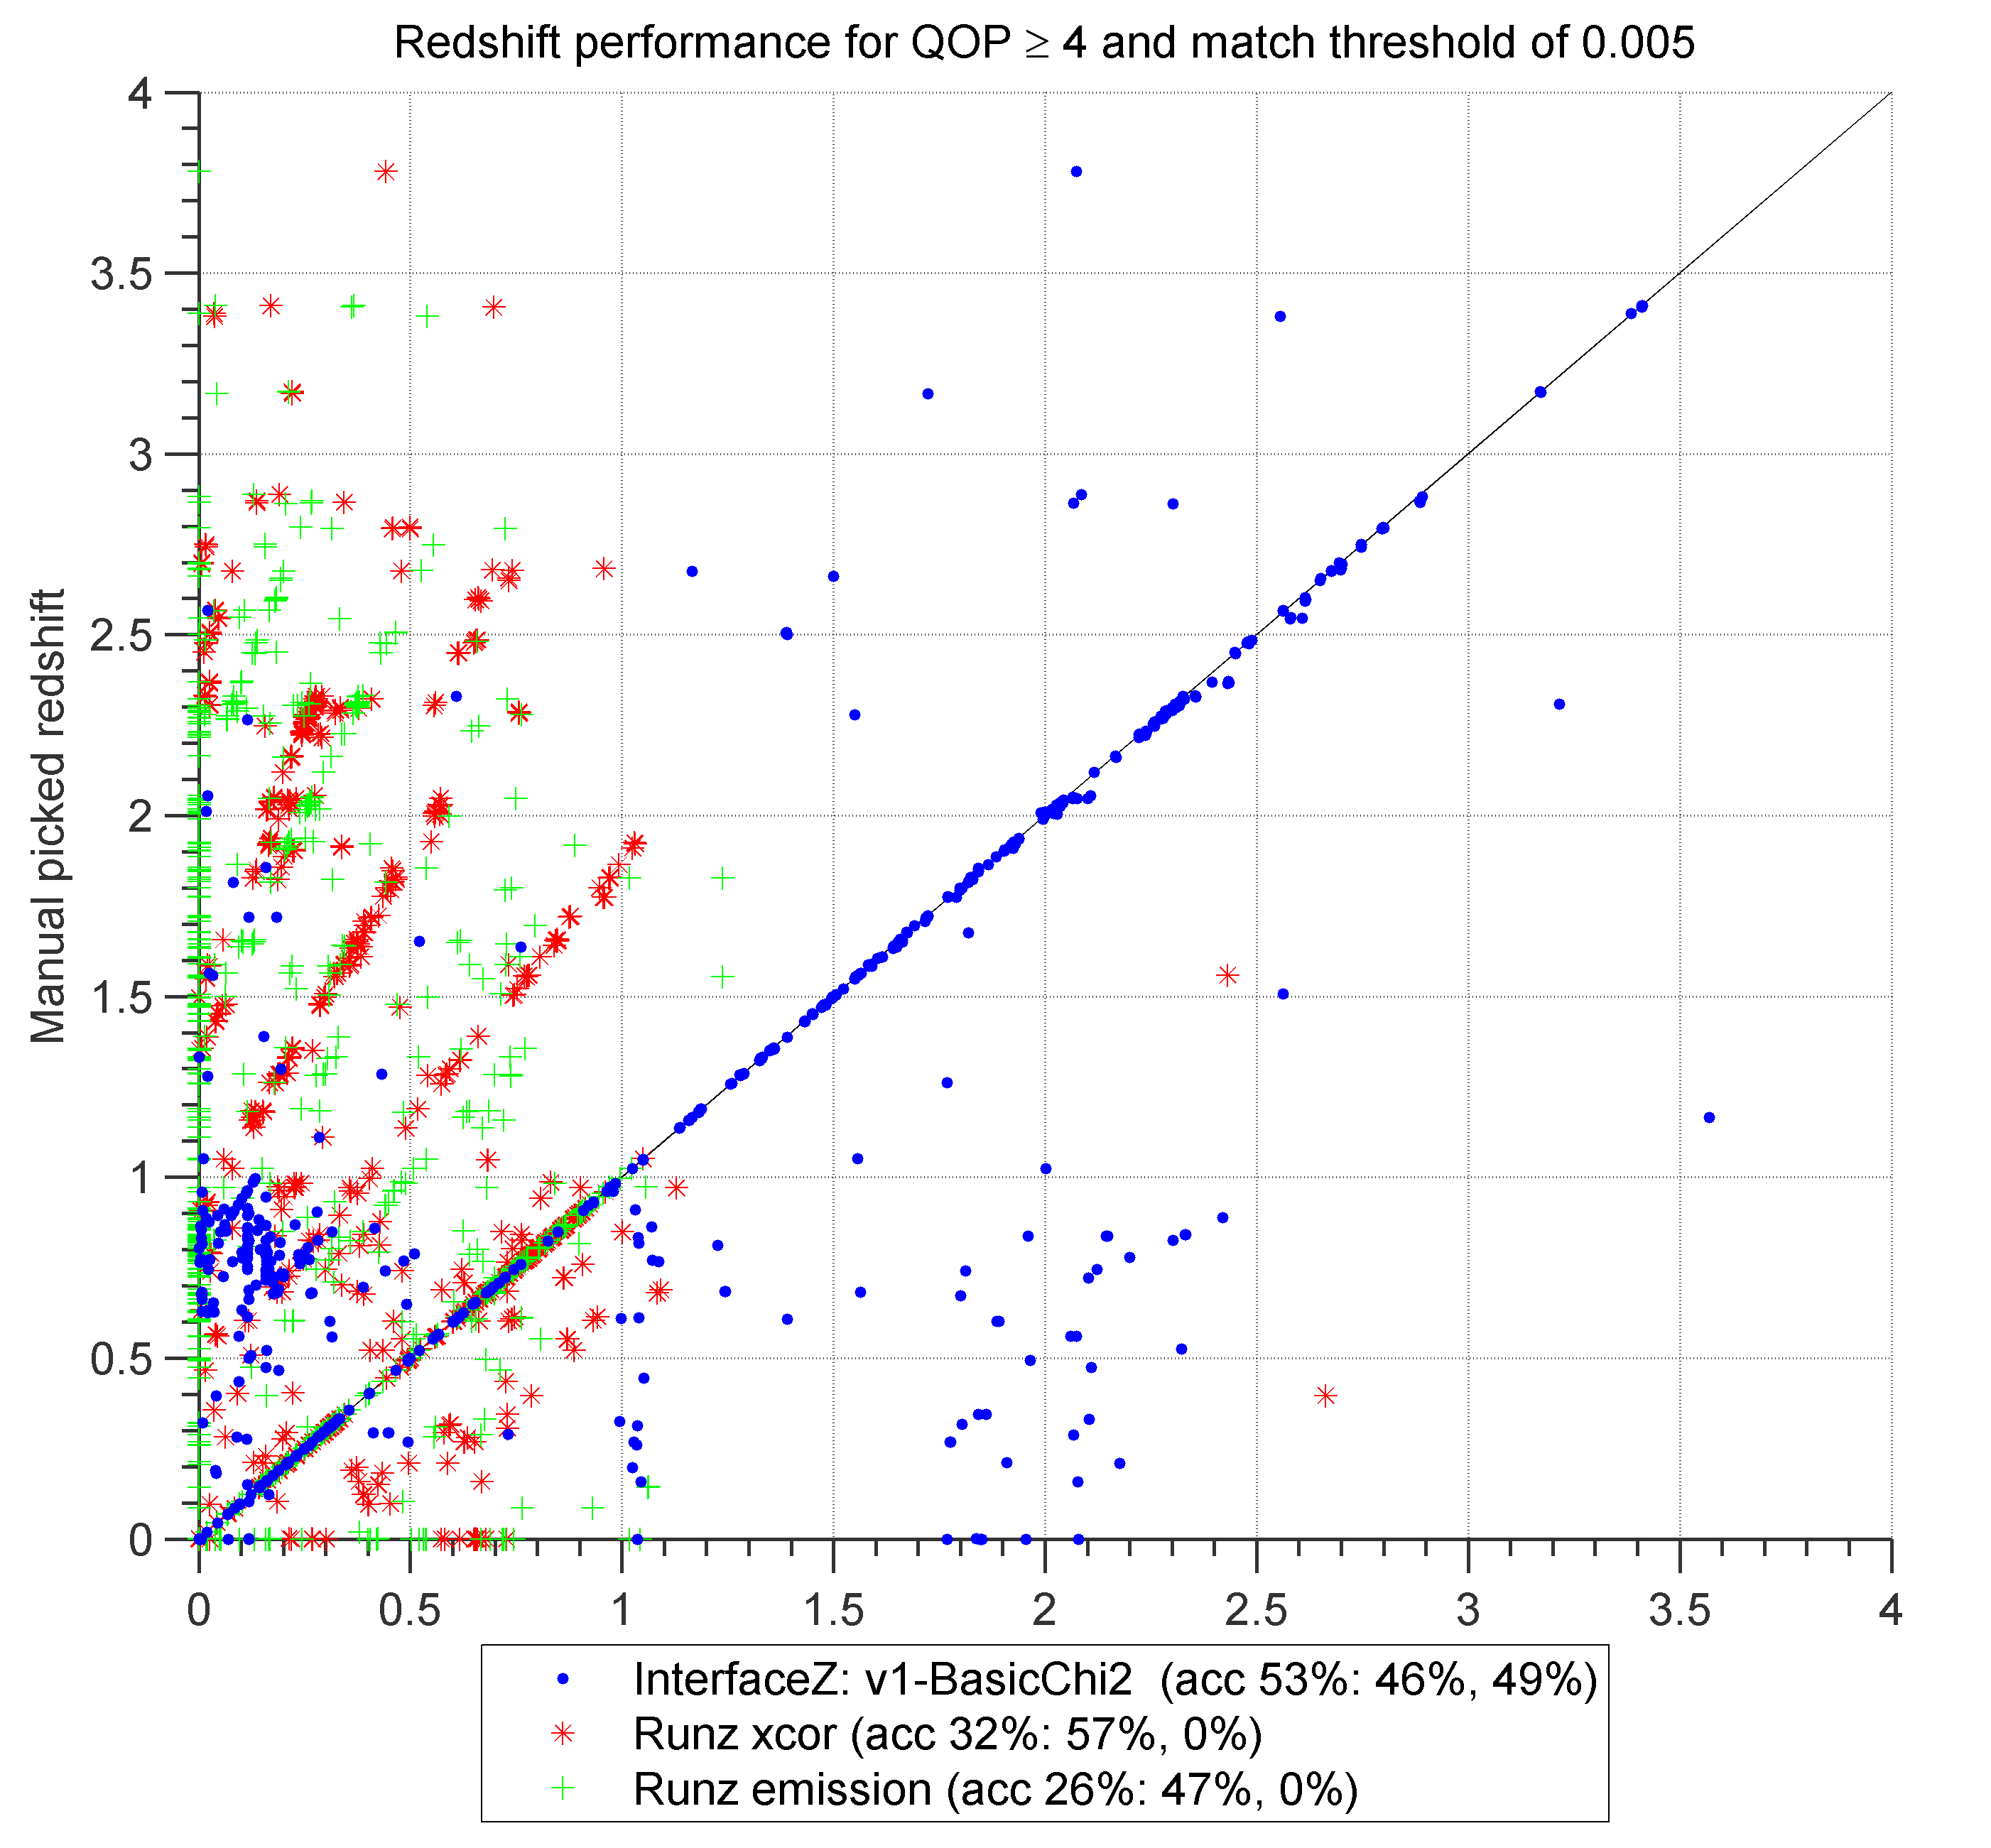
\includegraphics[width=0.9\textwidth]{images/Fullv1-BasicChi2.png} 
\centering
\caption{Comparison of manual redshifts with automatically determined redshifts by the unweighted $\chi^2$ algorithm and by the two algorithms in use with \runz{}. The first iteration of the $\chi^2$ matching algorithm is shown here, which used $w_i = \sqrt{\abs{s_i}}$ and $r = \brac{\sum_{i=1}^N s_i}^{5/2}$. Vertical result banding is still present at approximately $z=1$, which corresponds to minimal overlap of the galaxy templates, however it is decreased in intensity relative to Figure \ref{fig:vertical}.}
\label{fig:novertical}
\end{figure}

A better solution than a tailored reduction factor would be to simply increase the template lengths so that high redshift matches still have a significant portion of spectrum and template overlap. Unfortunately, the only templates found in research that went to sufficiently low wavelengths that overlap was no longer a problem were too low resolution to use for spectroscopic analysis. It was suggested by Professor Karl Glazebrook of Swinburne University to investigate BC12, PEGASE-HR or the Conroy models, however this has not been done to date given the success of the cross correlation algorithm with the existing templates.

\pagebreak
\section{Problems Encountered}

The decision to implement the thesis project in the most restricted, sandboxed and difficult language to work with certainly has benefits in accessibility and as a proof-of-concept for accessible scientific analysis via web applications, has caused a multitude of problems during development.

Perhaps the largest disadvantage to the web application approach is the security sandboxing which restricts all access to the client's file system unless the click explicitly passes a file into the web browser via drag-and-drop or a file upload dialogue. Part of the desired workflow for the thesis project was to designate a folder as the workspace, and automatically load in all FITs files, with their results, directly from this folder. Easily possible in any other language, this would require a user selecting the entire contents of the folder to be used every time they opened the web application. A HTML5 feature of the FileSystem API was going to be used to allow access to a restricted portion of the client's file system, however after development was begun, the FileSystem API development had to be discontinued and removed after Mozilla and Microsoft decided not to implement the API in April 2014 \cite{filesystem}. With this API gone, the only viable option was to have users manually select FITs files to upload to the web application for processing themselves.

The lack of file system access also complicated two other tasks apart from loading in FITs files: saving results and loading in results. Issues with saving results arise from the fact users download files off the web by the browser detecting HTTP headers on server response packets and recognising that the incoming response is a file to download rather than a web page to display. With no server side component to simulate such packets, and no ability to directly write to the while system, an alternate method of saving results had to be implemented. Whilst the HTML5 specification for the File Writer API does include the ability to save files from the client \cite{save1}, current browser implementation is not backwards compatible and is thus not sufficient for the task. A Javasciprt library, called FileSaver.js and written by Eli Grey, has implemented backwards compatibility for saving files \cite{save2}, and has thus been included as a library in the thesis project to allow downloading of text files in the client browser. Loading in of results was initially done the same way as loading a FITs file - drag-and-drop, however the ease at which a user could forget to drag in the results file and the extra step it added caused significant confusion in user testing. As such, it was decided that file results should never leave the browser, and with the availability of HTML5 local storage, up to five megabytes could be dedicated per site in the form of key-value data pairs \cite{local}. To minimise the space required to save the results, only the very final result for each spectrum is saved (as opposed to saving the top five best matches for example). The local storage has a wrapper service written so that the oldest spectrum are pruned out when approaching the five megabyte limit, however this would require having redshifted thousands of spectrum before hitting this limit.

The last large browser based impediment encountered was an inability to detect the number of CPU cores on client computers. As spectrum matching and preprocessing done on separate threads in the background, accurate detection of the number of CPU cores is a requirement for redshifting spectrum as fast as possible. Luckily, as of September 2, 2014, Google Chrome (version 37) implemented the \verb+navigator.hardwareConcurrency+ method \cite{chrome1,chrome2} which allows access to the number of logical processors in the clients machine. Prior to September, the number of cores had to be manually set on the settings page.

Scores of hours have also been dedicated to what should have been a simple task - page navigation. Whilst the chosen AngularJS routing plugin (UI Router) performed to specification, the redrawing of all page content on navigation causes a severe muli-second freeze when navigating back to the Overview page for large FITs files (as it requires up to 800 plots to be redrawn for a 400 spectrum file). Whilst this problem was solved early in the development of the application by using manual page routing, an application refactor and redesign saw the issue arise again. \textcolor{red}{PUT STUFF IN HERE WHEN YOU ACTUALLY FIX THE PROBLEM AGAIN}

The final large impediment encountered was organising the templates. The full template catalogue before refinement included all \runz{} templates, including those added by the WiggleZ cosmology team, and the Sloan Digital Sky Survey (SDSS) team. The large number of templates from the combined catalogues required a subset to be picked out that was representative of the objects being investigated, and this was done collaboratively with Tamara Davis, David Parkinson and Chris Lidman at the OzDES Busy Week gathering. In addition to this selection, problems with the template ranges (discussed in the previous section) were an impediment to high quality $\chi^2$ matching, and wider ranging templates of sufficient resolution could not be located. Finally, the largest template (the quasar template) was broken into pieces in the \runz{} application, and had to be manually stitched together and undergo manual normalisation in order to tune relative peak heights to achieve the greatest matching rate.





\chapter{Project Evaluation}




\section{Completion}



\begin{table}[ht!]
	\center
	\begin{tabular}{|c|c|c|}
		\hline
		Feature & Complete & Incomplete \\
		\hline
		Surface Capture & \gtick & \\
		Human interface (Control Panel) & \gtick & ple clients \\
		External control interface (RPC) & \gtick & \\
		ConSON Keystore) & \gtick & More settinurable \\
		Riagram recognition & \gtick & \\
		Block Diadel output \newline (MQTT Pubbscribe) & \gtick & \\
		Digital Logic Adapter & & \rcross \\
		Minimalist Digital Logic Simulator & & \rcross \\
		\hline
	\end{tabular}
	\caption{Feature completion for BlocSim prototype}
	\label{tab:completion}
\end{table} 

\newpage
%\clearpage



\section{Future Improvement}

Talk about what could be done in the future.
% =====================================================================

\chapter{Conclusion}

 This is my conclusion




























\chapter*{References}
\begingroup
\addcontentsline{toc}{chapter}{References}
\renewcommand{\addcontentsline}[3]{}
\renewcommand{\chapter}[2]{}
\bibliography{IEEEabrv,bibliography}
\endgroup


% =====================================================================

\end{document}
